\section{Méthodes de calcul bayésien}\label{calcul}

\subsection{Introduction}

Nous nous pla\c cons  dans le cadre à présent bien connu :
\begin{itemize}
\item Soit $\{X\sim f(.|\theta),\pi(\theta)\}$ un modèle bayésien servant à prendre une décision $\delta\in{\cal{D}}$. 
\item Dans un cadre d'\emph{\bf analyse ({\it a posteriori})}, on a observé des données ${\bf x_n}=(x_1,\ldots,x_n)\sim f(.|\theta)$.
\item La loi {\it a posteriori} $\pi(\theta|{\bf x_n})$ décrit l'ensemble des incertitudes sur $\theta\in\Theta$, vecteur inconnu qui ``paramétrise" l'état de nature.
\item Toute décision $\delta$ peut être jugée par un \emph{co\^ut} $L(\theta,\delta)$, c'est-à-dire son écart par rapport à une décision idéale inatteignable, affecté par la distribution de probabilité {\it a posteriori} $\pi(\theta|{\bf x_n})$.
\item La \emph{décision optimale} s'obtient en cherchant l'optimum de la fonction du co\^ut moyen {\it a posteriori} ({\it \emph{expected opportunity loss}}) : 
$\delta^{\pi}  =  \arg\min\limits_{\delta\in{\cal{D}}} R_B(\delta|\pi)$ avec
\begin{eqnarray*}
R_B(\delta|\pi) & = & \int_{\Theta} L(\theta,\delta) \ d\Pi(\theta|{\bf x_n}) \ = \ \int_{\Theta} L(\theta,\delta) \pi(\theta|{\bf x_n}) \ d\theta
\end{eqnarray*}
La question fondamentale du calcul bayésien est double : peut-on obtenir une expression explicite pour $\delta^{\pi}$ ? sinon, comment peut-on l'évaluer numériquement ? 
\end{itemize}

En général, l'estimateur de Bayes n'a pas de caractère explicite, car
\begin{eqnarray*}
\pi(\theta|{\bf x_n}) & = & \frac{f({\bf x_n}|\theta) \pi(\theta)}{\int f({\bf x_n}|\theta) \pi(\theta)d\theta }
\end{eqnarray*}
et le dénominateur n'est pas explicitement connu ($\pi(\theta|{\bf x_n})$ est définie à une constante d'intégration près). On peut essayer de l'estimer par \emph{intégration numérique} : les techniques classiques de Newton-Cotes ou Runge-Kutta mènent fréquemment à des instabilités numériques lorsque $\dim\Theta$ augmente. Toutefois, les méthodes de \emph{quadrature bayésienne} permettent de pallier ce problème. Elles relèvent encore du domaine de la recherche, et seront abordées plus tard dans ce cours.  \\

Fort généralement, le calcul d'estimateur de Bayes, mais aussi la sélection de modèle, la production de régions $\alpha-$crédibles (par exemple), nécessitent de pouvoir {\bf simuler {\it a posteriori}}. Par des techniques de Monte Carlo, %(voir $\S$ \ref{montecarlo} pour un rappel), 
fondée sur une capacité algorithmique de simulation pseudo-aléatoire (voir Annexe \ref{pseudoaleatoire}), on peut ainsi mener les calculs suivants :

\begin{enumerate}
    \item \emph{\bf Calcul d'une moyenne {\it a posteriori}}. On peut estimer $\delta^{\pi}$ par un { estimateur de Monte Carlo}
\begin{eqnarray*}
\hat{\delta}^{\pi}_M & = & \frac{1}{M} \sum\limits_{i=1}^M \theta_i 
\end{eqnarray*}
\begin{itemize}
\item Ingrédients : { Loi Forte des Grands Nombres ($\hat{\delta}^*_M \xrightarrow{p.s.}{} \delta^*$) + Théorème Central Limite}
\end{itemize}

\item \emph{\bf Estimation d'un quantile {\it a posteriori} d 'ordre $\alpha$}. On peut estimer $\delta^{\pi}$ par 
{ l'inversion de la fonction de répartition empirique} {\it a posteriori}
\begin{eqnarray*}
\hat{\Pi}_M(\theta|{\bf x_n}) & = & \frac{1}{M} \sum\limits_{i=1}^M \1_{\{\theta\leq {\theta^*_i}\}} \hspace{4cm} \text{ (Théorème de Glivenko-Cantelli)}
\end{eqnarray*}
%\begin{itemize}
%\item { Théorème de Glivenko-Cantelli : $\|\hat{\Pi}_M(\theta|{\bf x_n})-{\Pi}(\theta|{\bf x_n})\|_{\infty}\xrightarrow{\text{ unif.}}{} 0$}
%\end{itemize}
soit en prenant 
\begin{eqnarray*}
\hat{\delta}^{\pi}_M & = & \left\{ 
\begin{array}{lll} 
\frac{1}{2}\left(\theta^*_{\alpha\cdot M} + \theta^*_{\alpha\cdot (M+1)}\right) & & \text{si $\alpha\cdot M$ est entier} \\ 
\theta^*_{\lfloor\alpha\cdot{M}\rfloor +1} && \text{sinon}
\end{array} \right. \hspace{1.5cm} \text{ (Théorème de Mosteller)}
\end{eqnarray*}
\end{enumerate}

Un autre intérêt (et même une nécessité) apporté par la simulation {\it a posteriori} est le suivant : l'analyse prédictive. Plus précisément, pla\c cons-nous dans ce cadre :  {\bf simuler des réalisations de $X$} est une nécessité lorsqu'on s'intéresse au comportement $Y$ d'un phénomène (par exemple physique) modélisé ainsi :
\begin{eqnarray*}
Y & = & g(X,\nu) + \epsilon
\end{eqnarray*}
où :
\begin{itemize}
\item $g$ est une fonction (ou un code de calcul) {déterministe} ;
\item $\nu$ est un indice ou une variable indexant typiquement des conditions environnementales ;
\item $\epsilon$ est un ``bruit" stochastique qui modélise l'erreur entre la réalité du phénomène $Y$ et la sortie de $g$.
\end{itemize}
Dans ce problème de \emph{propagation d'incertitudes}, on cherche à reproduire un grand nombre de configurations de $Y$ pour calculer (par exemple) la probabilité que $Y$ dépasse un certain seuil. \\ 

\begin{exo}
$Y$ représente une hauteur d'eau aval, $g$ est un code hydraulique, $X$ est un débit d'eau amont, $\nu$ caractérise le frottement de la rivière et $\epsilon$ tient compte de la méconnaissance du terrain, de la précision du code, etc. \\
\end{exo}

\noindent Comment doit être simulé $X$ en entrée de $g$ ? La loi \emph{prédictive} de densité
\begin{eqnarray*}
f(x|{\bf x_n}) & = & \int f(x|\theta) \pi(\theta|{\bf x_n}) \ d\theta
\end{eqnarray*}
 permet de simuler une prochaine observation $x_{n+1}$ \emph{\it crédible} sachant qu'on a déjà observé les ${\bf x_n}$. Si l'on cherche à simuler de façon crédible la succession de {\bf deux} futures observations $(x_{n+1},x_{n+2})$, on doit procéder ainsi :
\begin{eqnarray*}
X_{n+1} & \sim &  f(x|{\bf x_n}), \\
X_{n+2} & \sim &  f(x|{\bf x_n},x_{n+1}), \ \ \ \text{etc.}
\end{eqnarray*}
Un algorithme simple de simulation repose donc sur la simulation de la loi {\it a posteriori}. \\

\begin{remark}{\bf Liens avec le \emph{machine /deep learning}.}
Les techniques de simulation et d'échantillonnage, dans le cadre spécifique du {\it machine / deep learning}, servent notamment  à : 
\begin{itemize}
\item initialiser des algorithmes d'optimisation de métriques, fonctions de coût complexes...; 
\item élaborer des {modèles génératifs}, tels les {\it Generative Adversarial Networks} (GAN) ; 
\item résoudre des problèmes de complétion de données manquantes ou en trop faible nombre ({\it data augmentation}) ; 
\item proposer des fa\c cons de sélectionner des mini-batchs utiles parmi un ensemble de données trop grand pour être processé intégralement {\it (problématique de plan d'expérience)} .
\end{itemize}

\end{remark}



%%%%%%%%%%%%%%%%%%%%%%%%%%%%%%%%%%%%%%%%%%%%%%%%%%
%\subsubsection{Rappels sur la méthode de Monte Carlo}\label{montecarlo}

%Les techniques de Monte Carlo repo



%%%%%%%%%%%%%%%%%%%%%%%%%%%%%%%%%%%%%%%%%%%%%%%%%%
\subsubsection{Principe de la simulation indirecte}

%\paragraph{Une simulation généralement indirecte.} Simuler selon la loi {\it a posteriori} $\pi(\theta|{\bf x_n})$ n'est en règle générale pas possible directement. Il faut donc utiliser des techniques qui font appel à de la \textcolor{black}{\bf simulation indirecte}:
\begin{enumerate}
\item on simule un tirage $\theta_{i}$ suivant une \emph{loi instrumentale} $\rho(\theta)$ (facile à simuler) ;
\item on utilise un \emph{test} pour déterminer si $\theta_{i}$ aurait également pu être un \emph{tirage plausible} de
$\pi(\theta|{\bf x_n})$.  
\end{enumerate}
Plus $\rho(\theta)$ est ``proche" de $\pi(\theta|{\bf x_n})$, plus ce test doit accepter les $\theta_{i}$. Plus précisément :
\begin{enumerate}
\item La densité $\rho(\theta)$ doit être facilement simulable (ex: mélanges gaussiens si $\pi(\theta|{\bf x_n})$ est multimodale...).  
\item Le \emph{support}\footnote{ \emph{Le domaine de $\Theta$ où la densité est non nulle.}} de $\rho(\theta)$ contient \emph{nécessairement} celui de $\pi(\theta|{\bf x_n})$.
\item Les queues de $\rho(\theta)$ devraient être plus lourdes que celles de $\pi(\theta|{\bf x_n})$.

\begin{center}
\vspace{-0.65cm}
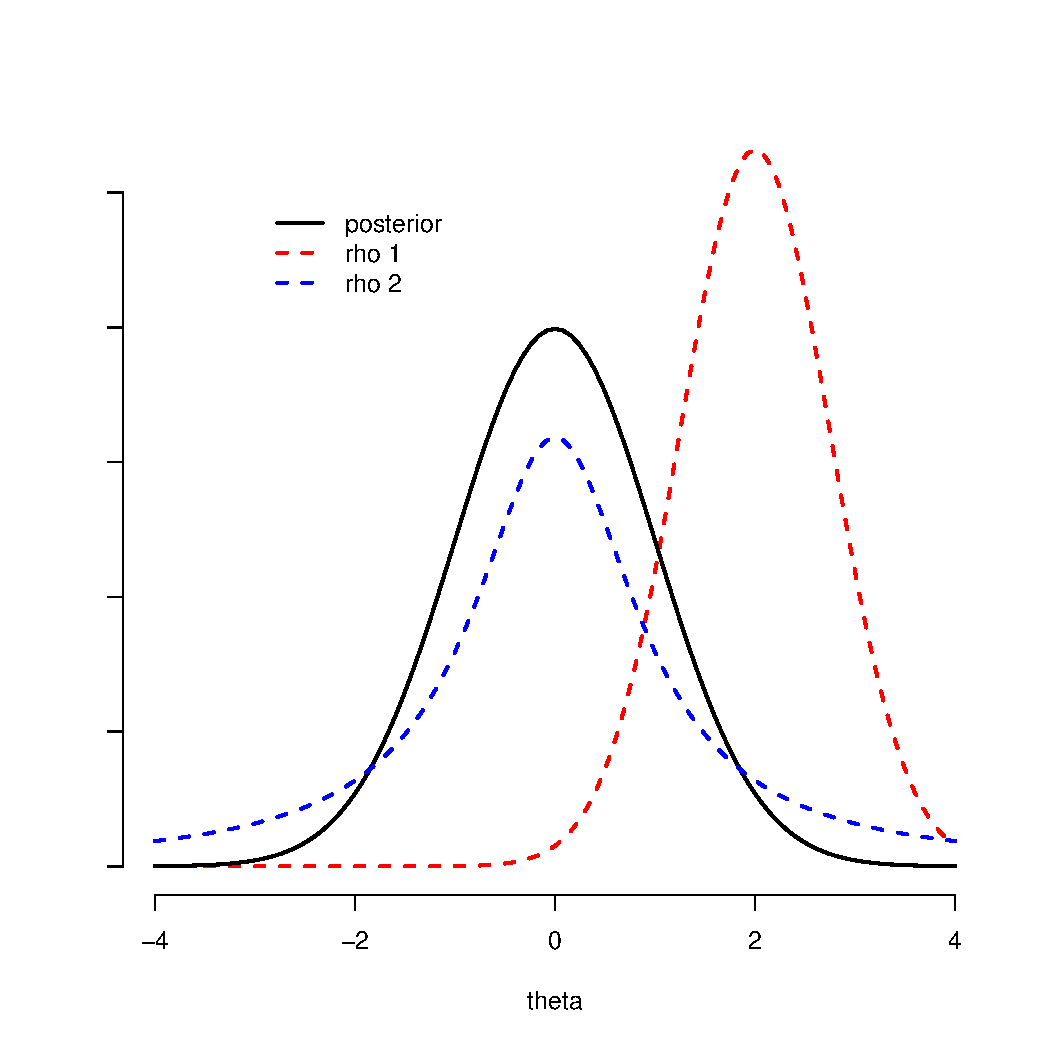
\includegraphics[scale=0.5]{figures/calcul/instrumentale.pdf}
\end{center}
\item Lorsque $\dim\Theta$ est petite (1 ou 2), on peut tracer $\pi(\theta|{\bf x_n})$ à un coefficient près pour sélectionner une forme intéressante pour $\rho(\theta)$.
\end{enumerate}
Un candidat logique peut parfois être la loi {\it a priori} $\pi(\theta)$, car elle respecte automatiquement la règle d'inclusion du support. Si l'{\it a priori} est très informatif par rapport aux données, l'{\it a posteriori} en sera proche. Une quantification de cette ``force" relative d'information est donc pratique pour choisir $\rho(\theta)$. Toutefois, ce choix peut être délicat : si l'{\it a priori} est très large (peu informatif), alors 
\begin{itemize}
\item il peut privilégier indûment des régions où la vraisemblance (comme fonction de $\theta$) est nulle ou quasi-nulle ;
\item  il faudra beaucoup de tirages pour atteindre les régions HPD (de plus haute densité) {\it a posteriori},  ce qui entraînera un  {coût algorithmique très fort}
\end{itemize}
Ce choix est aussi à proscrire si l'{\it a priori} privilégie des régions de $\Theta$ qui sont éloignées de celles privilégiées par les données. Une indication en faible dimension est de mesurer l'éloignement du mode {\it a priori} de $\theta$ et du maximum de vraisemblance $\hat{\theta}_n$. \\

\subsection{Méthodes d'échantillonnage dans la loi {\it a posteriori}}

Dans cette partie, on cherche doncà obtenir {\bf indirectement} des tirages qui suivent (en général approximativement) 
la loi {\it a posteriori}. Citons quelques algorithmes classiques que nous étudierons (quasiment tous) dans ce cours :
\begin{enumerate}
\item  algorithmes d'acceptation-rejet ;
\item  échantillonnage d'importance (préférentiel) ; 
\item  méthodes de Monte Carlo par chaînes de Markov (MCMC) ; 
\item  filtrage particulaire (pour les modèles à espace d'état).
\end{enumerate}
Ces méthodes  -- et leurs hybrides  -- sont les outils actuels les plus puissants pour simuler des lois connues semi-explicitement (à une constante/une intégrale près). Ils connaissent plusieurs approches d'\textbf{accélération} dont nous discuterons également, et qui amènent par ailleurs à faire un lien avec les techniques classiques du \emph{machine learning} : une technique de gradient stochastique, qui vise à estimer un mode {\it a posteriori} (et sous-entend en général que la loi {\it a posteriori} est approximativement gaussienne), peut être vue comme une forme dégénérée de MCMC adaptivement accélérée. \\

\subsubsection{Rappel : approches par inversion et transformations simples}

Rappelons avant de commencer que la méthode générique de simulation de $\theta\sim \pi(\theta|X)$ repose sur \emph{l'inversion de la fonction de distribution $\Pi$} qui, en unidimensionnel, est la fonction de répartition. \\

\begin{theorem}
Si $U\sim{\cal{U}}[0,1]$ et $\Pi(\theta|X)$ la fonction de répartition de $\theta|X$, alors $\Pi^{-1}(U|X)$ a la même loi que $\theta$.
\end{theorem}

La preuve vient du fait que par définition, $\Pi(\Pi^{-1}(U|X)\leq \theta|X)=\Pi(I\leq \Pi(\theta|X)|X)=\Pi(\theta|X)$. Si $\Pi$ n'est pas parfaitement croissante, on prend $\Pi^{-1}(u|X)=\inf\{\theta \ ; \ \Pi(\theta|X)\geq u\}$. \\



\begin{exo}
\begin{itemize} 
\item Loi binomiale ${\mathcal B}(n,p)$ : 
$
  F_X(x) = \sum_{i\le x} {n\choose i} p^i (1-p)^{n-i}
$
et $F_X^{-1}(u)$ s'obtient num\'eriquement.
\item  Loi exponentielle ${\mathcal E} (\lambda)$ :  
$
F_X(x) = 1 - \exp(\lambda x)$ et $
F_X^{-1}(u) = -\log({\textcolor{black}{\mathbf{u}}})/\lambda.
$
\item Loi de Cauchy ${\mathcal C} (0,1)$ : 
$
F_X(x) = \frac{1}{\pi} \arctan (x) + \frac{1}{2}$ et 
$ F_X^{-1}(u) = \tan(\pi({\textcolor{black}{\mathbf{u}}}-1/2))$. \\
.
\end{itemize}
\end{exo}

La critique de cette approche est aisée : $\Pi^{-1}(.|X)$ est rarement disponible, et ce ``théorème" (plutôt un lemme) d'inversion ne s'applique qu'en dimension 1. Pour "contrer" ces problèmes, on peut proposer quelques transformations (voir ci-dessous), mais cela ne permet de régler que des cas particuliers. \\

\begin{definition}{\bf Transformation de Box-M\"uller}
Pour la loi normale ${\mathcal N}(0,1)$, si $X_1,X_2\overset{iid}{\sim}{\mathcal N}(0,1)$, alors
$$
  X_1^2+X_2^2 \sim \chi^2_2, \qquad \arctan(X_1/X_2) \sim \mathcal{U}([0,2\pi]).
$$
%\rightline{\textcolor{black}{\sf[Jacobien]}}
Comme $\chi^2_2$ est identique \`a ${\mathcal E} (1/2)$, il vient par inversion :
$$
  X_1 = \sqrt{-2\,\log(U_1)} \,\sin (2\pi U_2)\qquad X_2 = \sqrt{-2\,\log(U_1)} \,\cos(2\pi U_2).
$$. 
\end{definition}

\noindent Les lois de Student et de Fisher se d\'eduisent naturellement
de la loi normale et de la loi du chi-deux. La loi de Cauchy se d\'eduit de la loi normale par la règle suivante : 
si $X_1,X_2\iid{\mathcal N}(0,1)$, alors $X_1/X_2 \sim {\mathcal C}(0,1)$. La loi Beta ${\mathcal B}_e(\alpha,\beta)$, de densit\'e
$$
  f_X(x) = \frac{\Gamma(\alpha+\beta)}{\Gamma(\alpha)\Gamma(\beta)}\,
	   x^{\alpha-1}(1-x)^{\beta-1}\,,
$$
s'obtient \`a partir de la loi gamma par la règle suivante : si 
$ X_1\sim {\mathcal G} a(\alpha,1)$, $X_2\sim {\mathcal G} a(\beta,1)$, alors
$$
  \frac{X_1}{X_1+X_2} \sim {\mathcal B}_e(\alpha,\beta). 
$$


\subsubsection{Simulation multidimensionnelle}\label{multidim.sim}

Le cas de la simulation multidimensionnelle est réglé également en principe par la règle en cascade suivante :

\begin{definition}{\bf Cascade rule.}
Supposons vouloir g\'en\'erer dans $\mathbb{R}^p$ l'échantillon 
$
(X_1,\ldots,X_p) \sim f(x_1,\ldots,x_p)
$
dont les composantes ne sont pas n\'ecessairement ind\'ependantes. La densité jointe s'écrit alors
$$
f(x_1,\ldots,x_p) = f_1(x_1)\times f_{2|1}(x_2|x_1)\ldots
\times f_{p|-p}(x_p|x_1,\ldots,x_{p-1}).
$$
On peut donc en déduire la règle d'implémentation suivante : \\

%{\makebox[0.5\textwidth][c]{\parbox{0.95\textwidth}{
\texttt{
Simuler pour $t=1,\ldots,T$
\begin{enumerate}
\item[1] {$X_1\sim f_1(x_1)$}
\item[2] {$X_2\sim f_{2|1}(x_2|x_1)$}
\item[ ] {$\vdots$}
\item[] {$X_p\sim f_{p|-p}(x_p|x_1,\ldots,x_{p-1})$}
\end{enumerate}
}
\end{definition}


\clearpage
\subsubsection{Algorithmes d'acception-rejet (AR)}

Ce type d'algorithme permet de simuler de façon {\bf exacte} et {\bf indépendante} selon la loi {\it a posteriori}. Il repose sur l'hypothèse suivante sur $\rho(\theta)$ :
$$
{\displaystyle 0 \ \ < \ \ K \ = \ \sup\limits_{\theta\in\Theta} \frac{f({\bf x_n}|\theta)\pi(\theta)}{\rho(\theta)} \ \ < \ \  \infty}.
$$

%\rule[0.5ex]{0.7\textwidth}{0.1mm} \\
 { \bf Algorithme AR:} \\
\rule[0.5ex]{0.7\textwidth}{0.1mm}
\vspace{-0.2cm}
\texttt{
\begin{enumerate}
\item { simulation indirecte :}  soit $\theta_i\sim \rho(\cdot)$ 
\vspace{0.05cm}
\item { test :} 
\begin{itemize} 
\item  soit $U_i\sim {\cal{U}}[0,1]$
\vspace{0.15cm}
\item  si ${\displaystyle U_i\leq \frac{f({\bf x_n}|\theta_i)\pi(\theta_i)}{K \rho(\theta_i)}}$ alors $\theta_i$ suit la loi $\pi(\theta|{\bf x_n})$
\end{itemize}
\end{enumerate}
\rule[0.5ex]{0.7\textwidth}{0.1mm}
}

\if\mycmdprooftwo1 \vspace{1cm} \begin{proof}%[Preuve] % Acceptation-rejet
Soit ${\theta}$ la variable aléatoire dont les tirages sont acceptées par le test. Alors, en définissant $P$ la mesure de probabilité usuelle sur $[0,1]$, et $\tilde{\Pi}$ la mesure de probabilité produit sur $\Theta\times[0,1]$, d'après la formule de Bayes,
\begin{eqnarray*}
\Pi\left(\tilde{\theta}\leq y | U \leq \frac{f({\bf x_n}|\theta)\pi(\theta)}{K\rho(\theta)} \right) & = & \frac{\tilde{\Pi}\left(\tilde{\theta}\leq y \ , \ U \leq \frac{f({\bf x_n}|\theta)\pi(\theta)}{K\rho(\theta)}\right)}{\tilde{\Pi}\left(U \leq \frac{f({\bf x_n}|\theta)\pi(\theta)}{K\rho(\theta)}\right)}, \\
& = & \frac{\int_{-\infty}^y \int_0^1 \frac{f({\bf x_n}|\theta)\pi(\theta)}{K\rho(\theta)} \ du \rho(\theta) \ d\theta}{\int_{-\infty}^{\infty} \int_0^{\frac{f({\bf x_n}|\theta)\pi(\theta)}{K\rho(\theta)}} \ du \rho(\theta) \ d\theta}, \\
& = & \frac{\int_{-\infty}^y f({\bf x_n}|\theta)\pi(\theta) \ d\theta}{K\int_{-\infty}^{\infty} \frac{1}{K}f({\bf x_n}|\theta)\pi(\theta) \ d\theta}, \\
& = & \Pi(\theta\leq y|{\bf x_n}).
\end{eqnarray*}
\end{proof}


\fi
\if\mycmdprooftwo0 {\it (Preuve en cours)}
\fi
\vspace{1cm}

Observons que la loi du nombre de tirages nécessaires selon $\rho(\theta)$ jusqu'à en accepter un suit la loi géométrique de probabilité $1/(K\cdot C)$ où $C$ est la constante d'intégration inconnue
\begin{eqnarray*}
C & = & \int_{\Theta} f({\bf x_n}|\theta)\pi(\theta) \ d\theta
\end{eqnarray*}
donc $K\cdot C$ est l'espérance du nombre de tirages nécessaires avant l'acceptation. \emph{Optimiser l'algorithme} revient donc à \emph{diminuer $K$}. 

\begin{exec}\label{quasi.conjug}
 On suppose $X   \sim {\cal{N}}(\theta,1)$ et on suppose connaître un échantillon ${\bf x_n}$ composé de :
\begin{itemize}
\item quelques observations $x_1,\ldots,x_{n-1}$ supposées iid. 
\item une pseudo-observation $y$ qui est un cas-limite masquant ({\it censurant}) une observation $x_{n}$ qui aurait dû être faite: $y<x_{n}$
\end{itemize}
 {\it A priori}, on suppose $\theta \sim {\cal{N}}(\mu,1)$. 
Pouvez-vous produire un algorithme d'AR qui génère des réalisations de la loi {\it a posteriori} de $\theta$ ? 
\end{exec}

\if\mycmdexotwo1 \vspace{1cm} \begin{rep}% AR
La vraisemblance s'écrit  
\begin{eqnarray*}
f({\bf x_n}|\theta) & \propto & \underbrace{\exp\left(-\frac{1}{2}\sum\limits_{k=1}^{n-1} (x_k-\theta)^2\right)}_{\text{\tiny terme régulier}} \ \ \ \left(\underbrace{1-\Phi(y-\theta)}_{\text{\tiny \begin{tabular}{l} terme dû à la censure \\ $\ \ = \ P(X>y)$ \end{tabular}}}\right).  
\end{eqnarray*}
L'{\it a posteriori} sur $\theta$ s'écrit alors
\begin{eqnarray*}
\pi(\theta|{\bf x_n}) & \propto & \tilde{\pi}(\theta|{\bf x_n}) \ = \ \exp\left\{-\frac{n}{2}\left[\theta - \frac{1}{n}\left(\mu + \sum\limits_{k=1}^{n-1} x_k\right)\right]^2\right\}\left\{1-\Phi(y-\theta)\right\}. 
\end{eqnarray*}
On remarque que si $y=x_n$, on aurait un modèle conjugué et $\pi(\theta|{\bf x_n})$ serait une loi normale. Il semble donc pertinent de proposer, comme choix de loi instrumentale,
$$
\rho(\theta) \equiv {\cal{N}}\left(\frac{1}{n}\left(\mu + \sum\limits_{k=1}^{n-1} x_k\right),1/n\right).
$$
Puisque $1-\Phi(y-\theta)\leq 1$, on a
\begin{eqnarray*}
\tilde{\pi}(\theta|{\bf x_n}) & \leq & \underbrace{\sqrt{\frac{2\pi}{n}}}_{K} \cdot\{1-\Phi(y-\theta)\}\cdot\rho(\theta).
\end{eqnarray*}
On peut donc mettre en oeuvre l'algorithme comme suit : on accepte $\theta_i$ si $U_i\leq 1-\Phi(y-\theta_i)$. Le nombre moyen d'appels nécessaires à $\rho(\theta)$ varie proportionnellement à $1/\sqrt{n}$, donc
plus l'échantillon de données grandit, plus l'algorithme est efficace.
Si cependant, on fait le choix $\rho(\theta)=\pi(\theta)$, alors
\begin{eqnarray*}
K & = & \sqrt{2\pi}\exp\left(\frac{1}{2}\left[\frac{1}{n-1}\sum\limits_{k=1}^n x_k - \mu\right](1-\sqrt{n})\right) 
\end{eqnarray*}
Voir la figure \ref{ARillus} pour une illustration de la mise en oeuvre de cet algorithme.
\end{rep}

\begin{figure}[hbtp]
\begin{center}
\includegraphics[scale=0.3]{figures/calcul/AR1.png} \\
\includegraphics[scale=0.3]{figures/calcul/AR2.png}
\caption{
Essai de simulation par AR en utilisant (en haut) une loi instrumentale ``proche" du vrai posterior ; (en bas) le prior comme loi instrumentale.}
\label{ARillus}
\end{center}
\end{figure}

\fi

\clearpage
\begin{exec}\label{gamma}
Soit un échantillon de loi gamma $x_1,\ldots,x_n\overset{iid}{\sim} {\cal{G}}(a,\theta)$ où $a$ est connu. On suppose $\pi(\theta)\equiv {\cal{G}}(c,d)$. Produisez une méthode par AR pour simuler la loi {\it a posteriori} $\pi(\theta|x_1,\ldot,x_n)$ et vérifiez que les tirages obtenus sont bien issus de cette loi, par ailleurs explicite.
\end{exec}

\if\mycmdexotwo1 \vspace{1cm} \begin{rep}
Il est aisé de vérifier qu'on connaît parfaitement la loi {\it a posteriori} de $\theta$ :
\begin{eqnarray*}
\theta|x_1,\ldots,x_n %& \sim & \pi(\theta|x_1,\ldots,x_n) \ \propto \ \\
& \sim & {\cal{G}}\left(c+an,d+\sum\limits_{i=1}^n x_i\right).
\end{eqnarray*}
On peut donc vérifier l'accord entre un échantillon iid simulé par AR et cette loi, via des tests statistiques classiques comme Kolmogorov-Smirnov, Cramer-von Mises ou Anderson-Darling. Pour construire cet algorithme d'AR, faisons par exemple le choix d'une loi instrumentale lognormale (qui est bien à support positif, car $\theta>0$) :
\begin{eqnarray*}
\rho(\theta|\mu,\sigma) & = & \frac{1}{\theta\sigma \sqrt{2\pi}} \exp\left(-\frac{1}{2\sigma^2}\left(\mu-\log\theta\right)^2\right).
\end{eqnarray*}
Il vient alors 
\begin{eqnarray*}
\kappa(\theta|\mu,\sigma)  \ = \  \frac{f(x_1,\ldots,x_n|\theta)\pi(\theta)}{\rho(\theta)} & = & {\displaystyle \frac{\sqrt{2\pi} \sigma \theta^{c+an} \exp\left(-\theta(d+\sum_{i=1}^n x_i)\right)}{\exp\left(-\frac{1}{2\sigma^2}\left(\mu-\log\theta\right)^2\right)}}
\end{eqnarray*}
et 
\begin{eqnarray*}
\frac{\partial }{\partial \theta} \log \kappa(\theta|\mu,\sigma) & = & \frac{c+an}{\theta} - \left(d+\sum\limits_{i=1}^n x_i\right) - \frac{1}{\sigma^2\theta}\left(\mu-\log(\theta)\right), \\
\frac{\partial^2 }{\partial \theta^2} \log \kappa(\theta|\mu,\sigma) & = & \frac{1}{\theta^2}\left(-(c+an) + \frac{1}{\sigma^2}(1+\mu - \log(\theta)\right).
\end{eqnarray*}
Notons $\theta_0(\mu,\sigma)=\exp(-(c+an)+(1+\mu)/\sigma^2)$. Si $0\leq \theta\leq \theta_0$, alors $\frac{\partial }{\partial \theta} \log \kappa(\theta|\mu,\sigma)$ est croissante. Si $\theta>\theta_0$, elle est décroissante vers $-(d+\sum_{i=1}^n x_i)<0$. Pour permettre à $\kappa(\theta|\mu,\sigma)$ d'être maximisable sur $\theta>0$, il faut donc que 
$$
\frac{\partial }{\partial \theta} \log \kappa(\theta_0(\mu,\sigma)|\mu,\sigma) = -\left(d+\sum\limits_{i=1}^n x_i\right) + 1/\sigma^2\theta_0 \ > \ 0.
$$
Sous cette contrainte, on peut résoudre numériquement en $\theta=\theta_1(\mu,\sigma)>\theta_0(\mu,\sigma)$ l'équation $\frac{\partial }{\partial \theta} \log \kappa(\theta|\mu,\sigma)=0$, et $\theta_1(\mu,\sigma)$ maximise alors $\kappa(\theta|\mu,\sigma)$. Dans ce cas, on peut définir 
\begin{eqnarray*}
K & = & \arg\min\limits_{\mu,\sigma} \kappa(\theta_1(\mu,\sigma)|\mu,\sigma). 
\end{eqnarray*}
et mettre en place l'algorithme AR.
\end{rep}
\fi

\begin{remark} On peut améliorer (faire baisser) le taux de rejet en encadrant la loi {\it a posteriori} entre 2 densités instrumentales 
 ({ acceptation-rejet par {\it enveloppe}}). \\
 \end{remark}
 
Le principe de l'AR est parfait en théorie, mais en pratique il est réservé aux cas simples ($\dim\Theta$ petite). De plus, cet algorithme est en général très coûteux en temps d'attente. 


\subsubsection{Algorithmes d'échantillonnage préférentiel ou d'importance (IS)}

Ce type d'algorithme vise surtout à produire un estimateur consistant d'une quantité d'intérêt {\it a posteriori}, mais il peut être utilisé dans un but de produire un échantillonnage exact mais non indépendant de la loi-cible (approche SIR). \\

{\bf Algorithme IS:} \\
\rule[0.5ex]{0.8\textwidth}{0.1mm}
\vspace{-0.2cm}
\texttt{
\begin{enumerate}
\item Soit $(\theta_1,\ldots,\theta_M)$ un tirage i.i.d. selon une densité instrumentale $\rho(\theta)$.
\item Soit $(\omega_1,\ldots,\omega_M)$ les {\bf poids d'importance} définis par
\begin{eqnarray*}
\omega_i & \propto &  \frac{f({\bf x_n}|\theta_i)\pi(\theta_i)}{\rho(\theta_i)}
\end{eqnarray*}
et normalisés de façon à ce que leur somme fasse 1.
\end{enumerate}
\rule[0.5ex]{0.8\textwidth}{0.1mm}
}

\begin{theorem}{Geweke 1989.}
Toute fonction {\it prédictive}
\begin{eqnarray*}
h(x|{\bf x_n}) & = & \int_{\Theta} h(x|\theta) \pi(\theta|{\bf x_n}) \ d\theta
\end{eqnarray*}
(ex: $h=f$) peut être estimée de façon consistante, lorsque $M\rightarrow\infty$, par
\begin{eqnarray*}
\hat{h}(x|{\bf x_n}) & = & \sum\limits_{i=1}^M \omega_i h(x|\theta_i).
\end{eqnarray*}
\end{theorem}

L'approche {\it Sampling-Importance Resampling} (SIR), proposée par Rubin (1988), se fonde sur le résultat suivant : 

\begin{theorem}\label{SIR.rubin}
Les tirages
\begin{eqnarray*}
\tilde{\theta}_1,\ldots,\tilde{\theta}_P & \sim & {\cal{M}}_{ultinomial}\left(\theta_1,\ldots,\theta_M|\omega_1,\ldots,\omega_M\right)
\end{eqnarray*}
suivent la loi {\it a posteriori} $\pi(\theta|{\bf x_n})$.
\end{theorem}

L'heuristique de Rubin consiste à prendre $P<M/20$ pour diminuer la dépendance dans l'échantillon resimulé. On peut aussi ainsi estimer les caractéristiques de $\pi(\theta|{\bf x_n})$ (moyenne, variance, etc.). \\

\begin{exo}
En reprenant une solution proposée pour l'exemple \ref{quasi.conjug}, par exemple $\rho(\theta) \equiv {\cal{N}}(\mu + \sum_{k=1}^{n-1} x_i,1/n)$, les poids sont simplement proportionnels à 
\begin{eqnarray*}
\omega_i & \propto & 1-\Phi(y-\theta_i)  
\end{eqnarray*}
qu'on normalise en divisant le membre de droite par la somme des $1-\Phi(y-\theta_i)$, $i=1,\ldots,M$. Les poids les plus hauts sont donc ceux pour lesquels $y \ll \theta_i$. \\
\end{exo}

Remarquons que fort logiquement, plus la densité instrumentale $\rho(\theta)$ est ``proche" de $\pi(\theta|{\bf x_n})$, plus les poids sont équilibrés (donc meilleur est le rééchantillonnage). Voir figure \ref{resume-IS} pour un résumé. Plutôt qu'une loi unique $\rho$, on peut mettre en place des algorithmes {\it adaptatifs} qui construisent itérativement une suite de densités $\{\rho_k(\theta)\}_k$ convergeant vers $\pi(\theta|{\bf x_n})$, pour améliorer encore le rééchantillonage. Une revue de tels algorithmes est proposée dans \cite{Marin2007}.   \\

\begin{figure}[h!]
\centering
\includegraphics[scale=0.3]{figures/calcul/is.png}
\caption{Schématisation du principe de l'échantillonnage d'importance.}
\label{resume-IS}
\end{figure}

Notons le résultat suivant, important et dû à Rubinstein (1981), qui guide ces recherches d'algorithmes IS optimaux. Ce résultat n'est pas exploitable directement, car il revient à avoir déjà résolu que l'on cherche à résoudre, mais il sert à construire des lois instrumentales qui progressivement vont se rapprocher de cette optimalité. 

\begin{theorem}{Importance sampling optimal.}
Soit l'estimateur de la fonction d'intérêt $h(\theta)\in\R$ par IS :
\begin{eqnarray*}
\hat{h}_M & = & \frac{1}{M}\sum\limits_{i=1}^M \frac{\pi(\theta_i|x)}{\rho(\theta_i)} h(\theta_i) \ \to \ \E_{\pi}[h(\theta|X] \ \ \ p.s.
\end{eqnarray*}
où les $\theta_i\overset{iid}{\sim} \rho(\theta)$. Alors le choix de $\rho$ qui minimise la variance de l'estimateur $\hat{h}_M$ est 
\begin{eqnarray*}
\rho^*(\theta) & = & \frac{|h(\theta)|\pi(\theta|X)}{\int_{\Theta}|h(\theta)|\pi(\theta|X) \ d\theta}.
\end{eqnarray*}
\end{theorem}

\if\mycmdprooftwo1 \vspace{1cm} \begin{proof}%[Preuve] % IS optimal
On note d'abord que
\begin{eqnarray*}
\V_{\rho}\left[\frac{h(\theta)\pi(\theta|x)}{\rho(\theta)}\right] & = & \E_{\rho}\left[\frac{h^2(\theta)\pi^2(\theta|x)}{\rho^2(\theta)}\right]-  \left(\E_{\rho}\left[\frac{h(\theta)\pi(\theta|x)}{\rho(\theta)}\right]\right)^2
\end{eqnarray*}
et que le second terme ne dépend pas de $\rho$. Il suffit donc de minimiser le premier terme. D'après l'inégalité de Jensen,  on a donc,
\begin{eqnarray*}
\E_{\rho}\left[\frac{h^2(\theta)\pi^2(\theta|x)}{\rho^2(\theta)}\right] & \geq & \left(\E_{\rho}\left[\frac{|h(\theta)|\pi(\theta|x)}{\rho(\theta)}\right]\right)^2, \\
& \geq & \left(\int_{\Theta} |h(\theta)|\pi(\theta|x) \ d\theta\right)^2
\end{eqnarray*}
qui est une borne inférieure indépendante de $\rho$, qui est atteinte en $\rho^*$.
\end{proof}
\fi
\if\mycmdprooftwo0 {\it (Preuve en cours)}
\fi
\vspace{1cm}



Un outil important, dès qu'on aborde le problème de la génération de données de même loi, mais corrélées, est la {\bf taille d'échantillon effective}, notée en général ESS (\emph{Effective Sample Size}). L'ESS relie la variance d'un estimateur de Monte Carlo idéal (échantillonnant directement dans la loi-cible) à la variance d'un estimateur fondé sur un échantillonnage corrélé, comme celui produit par l'IS, dans le cas où les deux estimateurs utilisent le même nombre de tirages. L'ESS mesure donc l'efficacité d'un algorithme d'échantillonnage corrélé. \\

\begin{definition}{\bf Effective Sample Size.}
Soit un échantillonnage instrumental $(\theta_1,\ldots,\theta_M)$ associé à des poids d'importance normalisés $(\omega_1,\ldots,\omega_M)$. Alors on définit
\begin{eqnarray*}
\mbox{ESS} & = & \left(\sum\limits_{i=1}^M \omega^2_i\right)^{-1}.
\end{eqnarray*}
\end{definition}

Lorsque l'échantillon produit est bien indépendant, les poids normalisés sont tous égaux à $1/M$, et donc $\mbox{ESS}=M^2/M=M$. \\

\begin{remark}
Dans le cas des MCMC, la définition précédente nécessite d'être remaniée pour tenir compte de la corrélation dans l'échantillonnage obtenu. \\
\end{remark}

Une autre propriété intéressante des techniques d'IS est de permettre de mener facilement certains types d'\textbf{analyse de sensibilité au prior}. Nous l'analysons dans l'exercice suivant.

\begin{exec}
Considérons une fonction d'intérêt $h(\theta)$ que l'on cherche à résumer par un estimateur calculé sous un coût quadratique ; il s'agit donc de l'espérance {\it a posteriori}
\begin{eqnarray}
h \ = \ \E_{\pi}[h(\theta)|x_1,\ldots,x_n] & = & \int_{\Theta} h(\theta)\pi(\theta|x_1,\ldots,x_n) \ d\theta\label{IS.estim1}
\end{eqnarray}
que l'on suppose pouvoir estimer simplement, de fa\c con consistante, par Monte Carlo. Supposons vouloir modifier le prior : $\pi(\theta)\to\pi'(\theta)$, sans modifier le support, mais de fa\c con à ce que la nouvelle loi {\it a posteriori} ne soit plus directement simulable. Peut-on (et sous quelles conditions) ne pas faire de calcul supplémentaire pour simuler le nouveau posterior $\pi'(\theta\x_1,\ldots,x_n)$ ?
\end{exec}

\if\mycmdexotwo1 \vspace{1cm} \begin{rep}
On considére donc une fonction d'intérêt $h(\theta)$ que l'on cherche à résumer par son espérance {\it a posteriori}
\begin{eqnarray}
h \ = \ \E_{\pi}[h(\theta)|x_1,\ldots,x_n] & = & \int_{\Theta} h(\theta)\pi(\theta|x_1,\ldots,x_n) \ d\theta\label{IS.estim1}
\end{eqnarray}
que l'on suppose pouvoir estimer simplement, de fa\c con consistante, par Monte Carlo :
\begin{eqnarray*}
\hat{h}_M & = & \frac{1}{M}\sum\limits_{k=1}^M h(\theta_i) \ \ \ \text{avec $\theta_i\overset{iid}{\sim} \pi(\theta|x_1,\ldots,x_n)$}
\end{eqnarray*}
Supposons vouloir modifier le prior : $\pi(\theta)\to\pi'(\theta)$, sans modifier le support, mais de fa\c con à ce que la nouvelle loi {\it a posteriori} ne soit plus directement simulable. En supposant que $\pi(\theta|x_1,\ldots,x_n)>0$ pour tout $\theta\in\Theta$, on peut néanmoins recalculer facilement le nouvel estimateur de Bayes :
\begin{eqnarray*}
h' \ = \ \E_{\pi'}[h(\theta)|x_1,\ldots,x_n] & = & \int_{\Theta} h(\theta)\pi'(\theta|x_1,\ldots,x_n) \ d\theta, \\
& = & \int_{\Theta} \omega(\theta_i) h(\theta)\pi(\theta|x_1,\ldots,x_n) \ d\theta
\end{eqnarray*}
avec
\begin{eqnarray*}
\omega(\theta_i) & = & \frac{\pi'(\theta|x_1,\ldots,x_n) }{\pi(\theta|x_1,\ldots,x_n)} \ = \ C\tilde{\omega}^*_i 
\end{eqnarray*}
où 
\begin{eqnarray*}
\tilde{\omega}^*_i  & = & \left(\frac{\pi'(\theta_i)}{\pi(\theta_i)}\right), \\
C & = &  \frac{m_{\pi}(x_1,\ldots,x_n)}{m_{\pi'}(x_1,\ldots,x_n)}.
\end{eqnarray*}
Le calcul de la constante de proportionnalité $C$ nécessiterait usuellement de disposer de deux échantillons {\it a posteriori}. On peut cependant s'en passer en remarquant que d'après la loi forte des grands nombres,  \begin{eqnarray*}
\frac{1}{M}\sum\limits_{i=1}^M \tilde{\omega}^*_i & \xrightarrow[n\to \infty]{p.s.} & \frac{1}{C}\int_{\Theta} \omega(\theta) \pi(\theta|x_1,\ldots,x_n) \ d\theta \ = \ 1/C
\end{eqnarray*}
et on en déduit donc qu'un estimateur IS  consistant de $h'$,  qui réutilise les calculs faits pour l'estimateur $\hat{h}_M$  sans coût calculatoire additionnel, est 
\begin{eqnarray*}
\hat{h''}_M & = & \frac{1}{M}\sum\limits_{k=1}^M \hat{\omega}^*_i h(\theta_i)
\end{eqnarray*}
avec
\begin{eqnarray*}
\hat{\omega}^*_i & = & \frac{\tilde{\omega}^*_i}{\sum\limits_{j=1}^M \tilde{\omega}^*_j}.
\end{eqnarray*}

 %\left(\frac{\pi'(\theta)}{\pi(\theta)}\right) \left(\frac{m_{\pi}(x_1,\ldots,x_n)}{m_{\pi'}(x_1,\ldots,x_n)}\right)
%\end{eqnarray*}
%Le second terme entre parenthèses ne dépend pas de $\theta$. En faisant l'hypothèse suivante :
%\begin{eqnarray*}
%\forall i\in\{1,\ldots,M\}, \ \ \pi(\theta_i_>0, \label{prior.pos}
%\end{eqnarray*}
%on peut donc proposer l'estimateur IS suivant pour $h'$, qui réutilise les calculs faits pour l'estimateur $\hat{h}_M$ : 
%\begin{eqnarray*}
%\hat{h'}_M & = & \frac{1}{M}\sum\limits_{k=1}^M \tilde{\omega}_i h(\theta_i)
%\end{eqnarray*}
%avec
%\begin{eqnarray*}
%\tilde{\omega}_i  =  C\tilde{\omega}^*_i & \text{et} & 
%\tilde{\omega}^*_i  =  \left(\frac{\pi'(\theta_i)}{\pi(\theta_i)}\right),
%\end{eqnarray*}
%et $C$ la constante de proportionnalité 
%\begin{eqnarray*}
%C & = & \frac{m_{\pi}(x_1,\ldots,x_n)}{m_{\pi'}(x_1,\ldots,x_n)}
%\end{eqnarray*}
%dont le calcul nécessite en théorie uniquement des tirages des deux priors (par Monte Carlo). Cependant, on remarque que par la loi forte des grands nombres, que 
%\begin{eqnarray*}
%\frac{1}{M}\sum\limits_{i=1}^M \tilde{\omega}^*_i & \xrightarrow[n\to \infty]{p.s.} & 
%\end{eqnarray*}

%On remarque, par la loi forte des grands nombres,  que

%\E\left[\frac{1}{M}\sum\limits_{i=1}^M \tilde{\omega}^*_i\right] \ = \ \frac{1}{M}\sum\limits_{i=1}^M \int_{\Theta} \pi'(\theta) \ d\theta \ = \ 1.
%\end{eqnarray*}
%Cependant, on sait que le calcul par Monte Carlo selon des tirages {\it a priori} du rapport $C$ des lois marginales peut être fortement instable. Il est donc simplement conseillé d'adopter la démarche suivante, suivant le théorème \ref{SIR.rubin} :
%\begin{enumerate}
%\item calculer les poids relatifs $\tilde{\omega}^*_i$ ;
%\item resimuler avec remise dans $\theta_1,\ldots,\theta_M$ selon les poids $\tilde{\omega}^*_i$ pour obtenir de nouveaux tirages {\it a posteriori} de $\pi'(\theta|x_1,\ldots,x_n)$. 
%\end{enumerate}
Notons que ce faisant, on crée de la corrélation entre les deux estimateurs de $h$. 
\end{rep}
\fi









\subsubsection{Méthodes de Monte Carlo par Chaînes de Markov (MCMC)}\label{MCMC}

Le principe des MCMC est de partir d'un tirage d'une densité $\tilde{\pi}_0(\theta)$ arbitraire, puis de 
produire une \emph{chaîne de Markov} de réalisations $\theta^{(1)},\ldots,\theta^{(M)}$ qui a pour loi
{\bf stationnaire} $\pi(\theta|{\bf x_n})$. \\ %Rappelons une série  de termes et résultats importants pour la construction et l'usage des MCMC. \\

\begin{definition}{\bf Noyau de transition.}
Une chaîne de Markov homogène est déterminée par un \emph{noyau de transition}, défini sur $\Theta\times {\cal{B}}(\Theta)$ à l'itération $i$ par 
\begin{eqnarray*}
{\cal{K}}(\theta|A) & = & P(\theta^{(i)}\in A | \theta^{(i-1)}=\theta) \ = \ \int_{A} \underbrace{{\kappa}(\theta,\tilde{\theta})}_{\text{\tiny densité de transition sur $\tilde{\theta}$}} \ d\tilde{\theta},
\end{eqnarray*} 
telle que ${\cal{K}}(.|A)$ est mesurable $\forall A \in {\cal{B}}(\theta)$. Cette notion de noyau généralise au cadre continu celle de matrice de transition d'un état à un autre dans un cadre discret. 
\end{definition}

\noindent Toute la structure d'une chaîne de Markov, que l'on considèrera toujours d'ordre 1 dans ce cours, dépend seulement du choix d'un noyau de transition et de l'état initial (ou la distribution initiale) de la chaîne, comme l'exprime la définition suivante. 

\begin{definition}{\bf Chaîne de Markov.}
 Sachant un noyau de transition ${\cal{K}}$, une suite $\theta_0,\ldots,\theta_n,\ldots$ de variables aléatoires est une chaîne de Markov d'ordre 1 si, $\forall n\geq 0$, la distribution de $\theta_n$ conditionnelle à la $\sigma-$algèbre (filtration) générée par $\theta_{n-1},\theta_{n-2},\ldots,\theta_0$ est la même que celle de $\theta_{n}|\theta_{n-1}$ :
 \begin{eqnarray*}
 \pi\left(\theta_n\in {\cal{A}} | \theta_{n-1},\theta_{n-2},\ldots,\theta_0\right) & = & \pi\left(\theta_n\in {\cal{A}} | \theta_{n-1}\right), \ 
 = \  {\cal{K}}(\theta_{n-1}|{\cal{A}}).
 \end{eqnarray*}
\end{definition}

\noindent Des éléments fondamentaux de théorie des chaînes de Markov sont rappelés en Annexe \ref{markovtheory}. Nous en retenons surtout un résultat fondamental, le \emph{théorème ergodique}. Celui-ci nous donne "le droit", sous certaines conditions, de mener des calculs de Monte Carlo à partir de chaînes de valeurs corrélées produites par une chaîne de Markov. On parlera alors de méthode de Monte Carlo par chaîne de Markov (MCMC).  

\begin{theorem}{\bf (Théorème ergodique).}\label{theorem.ergogique}
Si la chaîne de Markov $(\theta_n)_{n\geq 0}$ est réccurente positive\footnote{Plus précisément Harris-récurrente positive, cf. Annexe \ref{markovtheory}.}, alors pour toute fonction $h:\Theta\to\R$ telle que $\E_{\pi}[|h| \ | x_1,\ldots,x_n] ]<\infty$, alors
$$
\lim\limits_{n\to\infty} \frac{1}{n} \sum\limits_{i=1}^n h(\theta_i)  =  \int_{\Theta} h(\theta) \ d\Pi(\theta|x_1,\ldots,x_n).
$$
Si de plus la chaîne $(\theta_n)_{n\geq 0}$ est réversible, alors 
\begin{eqnarray*}
\frac{1}{\sqrt{n}} \sum\limits_{i=1}^n \left(h(\theta_i)-\E_{\pi}[h  | x_1,\ldots,x_n] \right) & \xrightarrow[n\to\infty]{{\cal{L}}} & {\cal{N}}(0,\gamma^2)
\end{eqnarray*}
avec
$$
0 \ < \ \gamma^2 = \E_{\pi}\left[h^2(\theta_0)  | x_1,\ldots,x_n\right] + 2 \sum\limits_{k=1}^{\infty} \E_{\pi}\left[h(\theta_0) h(\theta_k)  | x_1,\ldots,x_n\right] \ < \ \infty.
$$
\end{theorem}


\paragraph{Caractéristiques générales d'une MCMC.}
\`A l'itération $i$ d'une MCMC, la densité de probabilité d'un $\theta$ simulé est
$$
\tilde{\pi}_i(\theta)  =  \int_{\hat{\theta}\in\Theta} \tilde{\pi}_{i-1}(\hat{\theta}) {\kappa}(\hat{\theta},\theta) \ d\hat{\theta}
$$
et converge en loi vers une \emph{unique densité stationnaire $\tilde{\pi}_{\infty}(\theta)$}, indépendamment de $\tilde{\pi}_0$, sous des conditions très générales de convergence et d'unicité :
\begin{itemize}
\item tout état (ou sous-ensemble) de $\Theta$ est accessible à partir de n'importe quel autre état  ({\it irréductibilité}) ;
\item le nombre minimal d'états intermédiaires est nul  ({\it apériodicité}) ; cela se traduit, lorsque $\Theta$ est discret, par le fait que la chaîne ne peut pas boucler sur un ensemble d'états ; 
\item l'espérance du temps de retour en n'importe quel état est fini ({\it récurrence positive}).
\end{itemize}
Les caractéristiques majeures d'une MCMC sont les suivantes (cf. figure \ref{ex-mcmc-1}) :
\begin{itemize}
\item le début de la chaîne (dit \emph{\it temps de chauffe}) sert à explorer l'espace $\Theta$ et trouver les zones de {\bf haute densité {\it a posteriori}} ;
\item on ne conserve que la seconde partie de l'ensemble des $\theta^{(i)}$ produits, qui suivent la distribution stationnaire (la chaîne ``oublie" son état initial) ; 
\item la fréquence de visite de chaque état (ou sous-ensemble) de $\Theta$ est la même pour toute trajectoire MCMC ; 
\item on ajoute souvent une étape de \emph{rééchantillonage} (SIR) ou de \emph{décorrélation} des $\theta^{(i)}$ conservés pour obtenir
un échantillon approximativement indépendant de $\tilde{\pi}_{\infty}(\theta)$.  \\
\end{itemize} 





\paragraph{Application au bayésien.}
Si on veut appliquer le principe des MCMC au bayésien, il faut que la loi stationnaire $\tilde{\pi}_{\infty}(\theta)$ soit la loi {\it a posteriori} $\pi(\theta|{\bf x_n})$. Pour cela, le noyau ${\cal{K}}$ doit être construit en fonction de la vraisemblance des données ${\bf x_n}$ et de l'{\it a priori} $\pi(\theta)$. On peut prosa\"iquement réutiliser la structure de  l'algorithme d'Acceptation-Rejet, en créant un noyau résultant du mélange de deux actions à l'itération $i$ :
\begin{itemize}
\item on accepte un nouveau candidat-tirage de $\tilde{\pi}_i(\theta)$ avec une probabilité $\alpha_i$ ;
\item on refuse et on conserve le tirage précédent dans la chaîne avec probabilité $1-\alpha_i$.
\end{itemize}
Ce type d'algorithme a été formalisé et est connu sous le nom d'\textbf{algorithme de Hastings-Metropolis} (HM). Sous certaines conditions de conditionnement explicite {\it a posteriori}, on peut accepter des candidats avec probabilité $1$. Ceci donne une forme particulière de MCMC, connue sous le nom d'\textbf{algorithme de Gibbs}. \\

\paragraph{Algorithme HM.} La structure de l'algorithme est la suivante. \\%Soit une densité instrumentale $\rho(\theta|\theta^{(i-1)})$.

\texttt{\'Etape $i$: \\
\rule[0.5ex]{0.8\textwidth}{0.1mm}
\vspace{-0.2cm}
\begin{enumerate}
\item Simuler selon une loi instrumentale $\tilde{\theta} \sim \rho(\theta|\theta^{(i-1)})$.
\item Calculer la probabilité 
\begin{eqnarray*}
\alpha_i & = & \min\left\{1,\left(\frac{f({\bf x_n}|\tilde{\theta})\pi(\tilde{\theta})}{f({\bf x_n}|{\theta^{(i-1)}})\pi({\theta^{(i-1)}})}\right)\cdot\left(\frac{\rho(\theta^{(i-1)}|\tilde{\theta})}{\rho(\tilde{\theta}|\theta^{(i-1)})}\right)\right\}.
\end{eqnarray*}
\item $\left.\begin{tabular}{l}
\text{Simuler $U\sim{\cal{U}}_{\text{\tiny unif}}[0,1]$}. \\
\\
\text{Si $U\leq \alpha_i$ choisir $\theta^{(i)}=\tilde{\theta}$}. \\
\text{Sinon choisir $\theta^{(i)}=\theta^{(i-1)}$}. 
\end{tabular}\right\}$ Accepter $\tilde{\theta}$ avec probabilité $\alpha_i$. 
\end{enumerate}
\rule[0.5ex]{0.8\textwidth}{0.1mm}
}

\vspace{0.5cm}

Le noyau markovien est alors constitué d'un mélange d'un Dirac en $\theta^{(i-1)}$ et de la loi instrumentale, mélange pondéré par la probabilité de transition $\alpha_i$. La partie continue
du noyau de transition (de $\theta$ vers $\theta'$) s'écrit
\begin{eqnarray*}
p(\theta,\theta')  & = & \alpha(\theta,\theta')\rho(\theta'|\theta)
\end{eqnarray*}
avec $\alpha(\theta,\theta')$ la probabilité de transition
\begin{eqnarray*}
\alpha(\theta,\theta') & = & \min\left\{1,\left(\frac{f({\bf x_n}|\theta')\pi(\theta')}{f({\bf x_n}|{\theta})\pi(\theta)}\right)\cdot\left(\frac{\rho(\theta|\theta')}{\rho(\theta'|\theta)}\right)\right\}.
\end{eqnarray*}
On a  
\begin{eqnarray*}
\pi(\theta) \times p(\theta,\theta')  & = & \pi(\theta') \times p(\theta',\theta).
\end{eqnarray*} 
La chaîne MCMC produite est alors dite \emph{réversible} et ceci suffit à montrer, si la chaîne est irréductible et  apériodique, que :
\begin{itemize}
\item elle est ergodique ; 
\item la distribution des itérés $\theta^{(i)},\ldots,\theta^{(j)}$ de la chaîne converge en loi vers une loi-limite unique ; 
\item celle-ci est proportionnelle à $f({\bf x_n}|\theta)\pi(\theta)$ : il s'agit donc de $\pi(\theta|{\bf x_n})$.
\end{itemize}
L'irréductibilité peut être facilement assurée par la contrainte suivante : le support de la loi instrumentale doit inclure le support de la loi-cible. \\

Le rapport de Metropolis fait intervenir le rapport des lois {\it a posteriori} (qui permet d'\^oter la constante d'int\' egration inconnue) : à l'étape $k$, si $\tilde{\theta}_{k}$ se situe plus haut dans la  zone de haute densit\' e de $\pi(\theta|{\bf x_n})$ que $\theta_{k-1}$, ce rapport est plus grand que 1. Le rapport inverse des lois instrumentales et l'usage d'un tirage uniforme interdisent d'automatiser l'acceptation de ce nouveau point, en permettant \`a la cha\^ine de Markov d'explorer exhaustivement l'espace $\Theta$. \\




\begin{exec}\label{debit.extreme}
Soit $X$ la variable ``débit maximal de rivière". Elle est supposée suivre une loi des extrêmes (Gumbel) de densité
\begin{eqnarray*}
f(x|\theta) & = &  \lambda\mu\exp(-\lambda x)
\exp(-\mu\exp(-\lambda x)).
\end{eqnarray*}
avec $\theta=(\mu,\lambda)$. %L'espérance est
%\begin{eqnarray*}
%\E[X|\theta] & = & \lambda^{-1}\left(\log \mu + \gamma\right)
%\end{eqnarray*}
%où $\gamma$ est la constante d'Euleur ($\simeq$ 0.578..)
\begin{center}
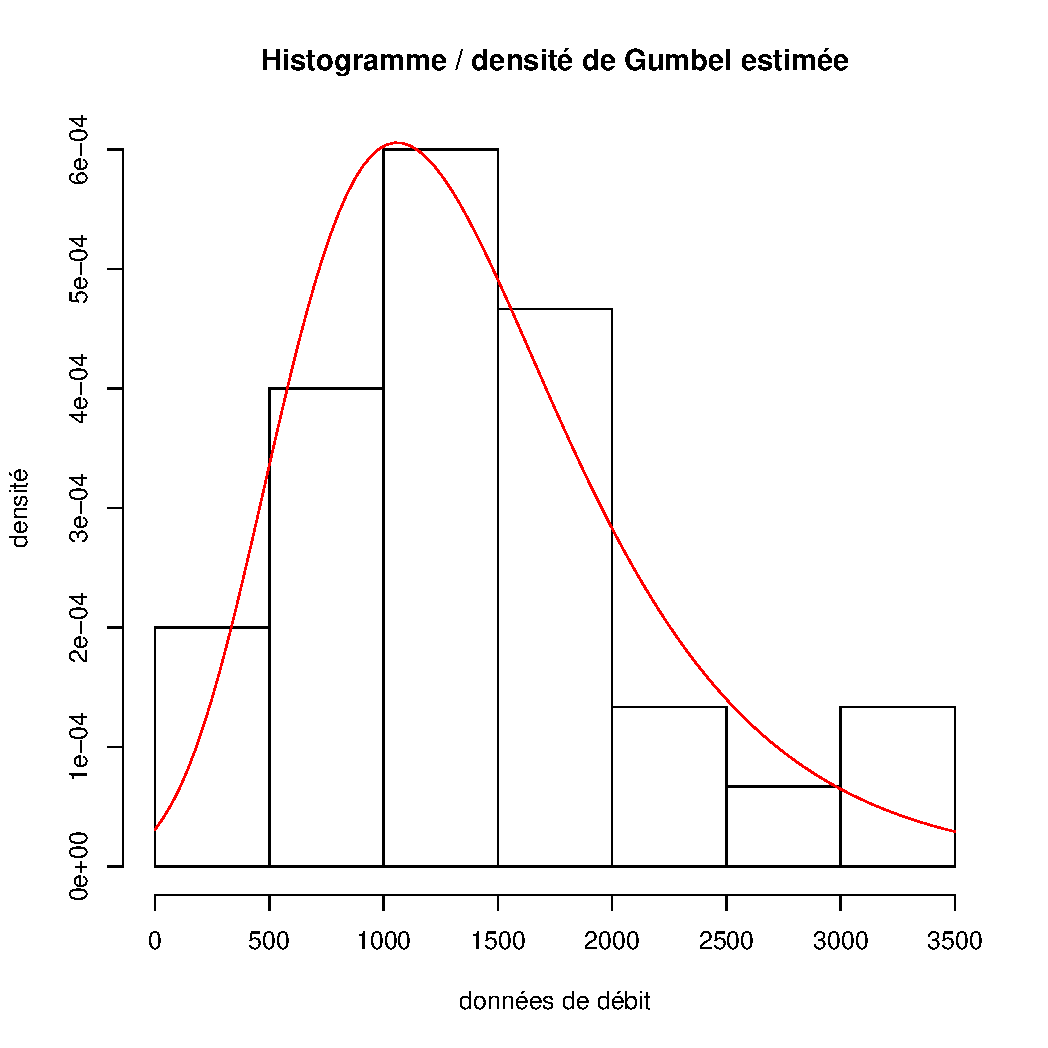
\includegraphics[scale=0.4]{figures/calcul/hist-gumbel.pdf}
\end{center}
Considérons $n$ observations ${\bf x_n}=(x_1,\ldots,x_n)$ supposées iid  selon cette distribution. 
\begin{enumerate}
    \item Comment s'écrit la vraisemblance ?
    \item On considère l'{\it a priori} $\pi(\mu,\lambda) = \pi(\mu|\lambda)\pi(\lambda)$ avec
\begin{eqnarray*}
\mu|\lambda & \sim   & {\cal{G}}\left(m,b_m(\lambda) \right),  \\
\lambda    & \sim   & {\cal{G}}\left(m,m/\lambda_e\right)
\end{eqnarray*}
et ${\displaystyle b_m(\lambda)  = \left[\alpha^{-1/m}
-1\right]^{-1} \exp(-\lambda x_{e,\alpha}).}$. Ces hyperparamètres ont le sens suivant :
\begin{itemize}
\item $x_{e,\alpha}=$ quantile prédictif {\it a priori} d'ordre $\alpha$:
\begin{eqnarray*}
P\left(X<x_{e,\alpha}\right) & = & \int P\left(X<x_{e,\alpha}|\mu,\lambda\right)  \pi(\mu,\lambda) \ d\mu d\lambda \ = \ \alpha ; 
\end{eqnarray*}  
\item $m =$ taille d'échantillon fictif, associée à la ``force" de la connaissance {\it a priori} $x_{e,\alpha}$ ; 
\item $1/\lambda_e = $ moyenne de cet échantillon  fictif. 
\end{itemize}
Pouvez-vous produire un algorithme de type MCMC qui permette de générer une loi jointe {\it a posteriori} pour $(\mu,\lambda)$ ? 
\end{enumerate}
\end{exec}

\if\mycmdexotwo1 \vspace{1cm} \begin{rep}
En posant
%\begin{eqnarray*}
$\bar{x}_n  =  \frac{1}{n}\sum\limits_{i=1}^n x_i$ et 
$\bar{b}_{{\bf x_n}}(\lambda)  =  \sum\limits_{i=1}^n \exp\left(-\lambda x_i\right)$, 
la vraisemblance s'écrit alors
\begin{eqnarray*}
f\left({\bf x_n}\right) & = & \lambda^n \mu^n \exp(-\lambda n\bar{x}_n) \exp\{-\mu\bar{b}_{{\bf x_n}}(\lambda)\}.
\end{eqnarray*}
En conséquence, la loi {\it a posteriori} s'obtient sous la forme \emph{hiérarchisée} suivante :
\begin{eqnarray*}
\pi\left(\mu,\lambda|{\bf x_n}\right) & = & \pi\left(\mu|\lambda,{\bf x_n}\right) \pi\left(\lambda|{\bf x_n}\right)
\end{eqnarray*}
où
\begin{eqnarray*}
\mu|\lambda,{\bf x_n} & \sim & {\cal{G}}\left(m+n,b_m(\lambda) + \bar{b}_{{\bf x_n}}(\lambda)\right)
\end{eqnarray*}
et
\begin{eqnarray*}
\pi\left(\lambda|{\bf x_n}\right) & =  & %\underbrace{\propto}_{\text{\tiny proportionnel}} &  
\gamma(\lambda)\cdot {\cal{G}}\left(m+n,{m}/{\lambda_e} + n\bar{x}_n\right)
%\frac{\left(b_m(\lambda)\right)^m}{\left(b_m(\lambda) + \bar{b}_{{\bf x_r},{\bf c_{n-r}}}(\lambda)\right)^{m+r}} \lambda^{m+r-1} \exp\left(-\lambda ({m}/{\lambda_e} + r\bar{x}_r) \right)
\end{eqnarray*}
avec
\begin{eqnarray*}
\gamma(\lambda) & \propto & \frac{b^m_m(\lambda)}{ \left(b_m(\lambda) + \bar{b}_{{\bf x_n}}(\lambda)\right)^{m+n}}
\end{eqnarray*}
La loi {\it a priori} est donc \emph{semi-conjuguée}, et il suffit de simuler $\lambda$ {\it a posteriori} pour obtenir un tirage joint {\it a posteriori} de $(\mu,\lambda)$. On trace ci-dessous quelques graphiques typiquement obtenus. Plusieurs choix de lois instrumentales pour $\rho(\lambda|\lambda^{(i-1)})$ peuvent être faits. On peut notamment proposer : 
\begin{itemize}
\item la loi {\it a priori} $\pi(\lambda)$ ; 
\item une loi qui ``semble proche": ${\cal{G}}\left(m+n,{m}/{\lambda_e} + n\bar{x}_n\right)$ ; 
\item une loi normale de moyenne $\lambda^{(i-1)}$ et de coefficient de variation petit (5\%) ou grand (25 ou 50\%).
\end{itemize}


\begin{center}
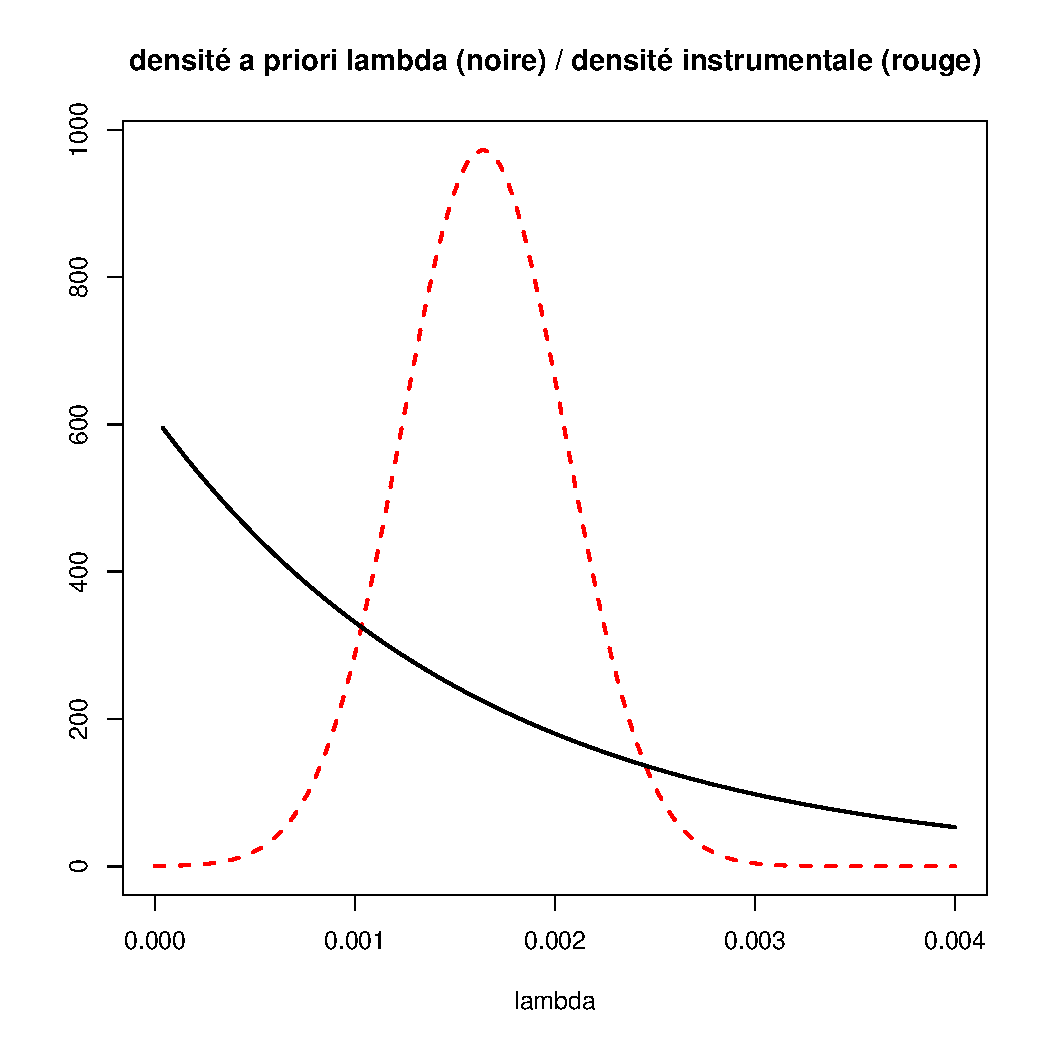
\includegraphics[width=6cm,height=5cm]{figures/calcul/prior-1.pdf} 
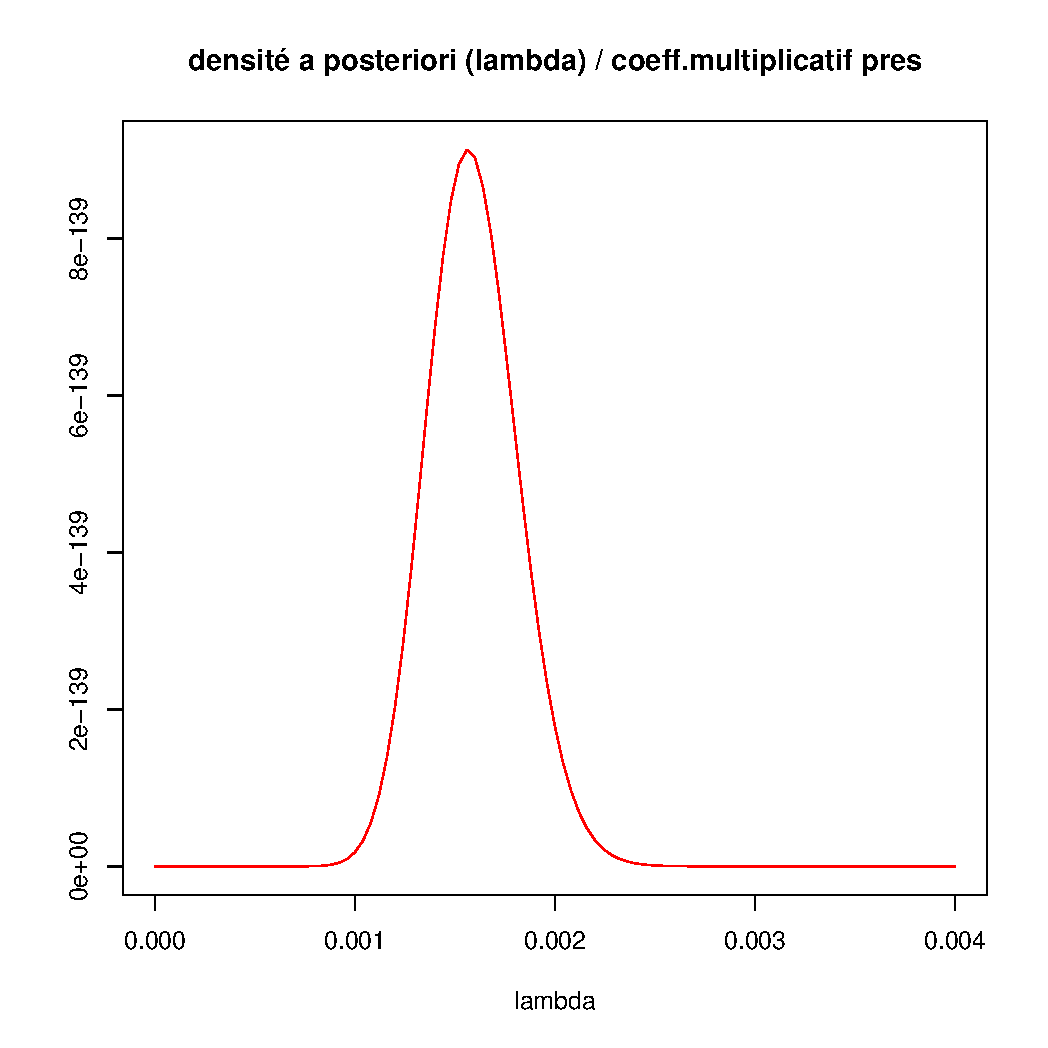
\includegraphics[width=6cm,height=5cm]{figures/calcul/posterior-1.pdf} \\
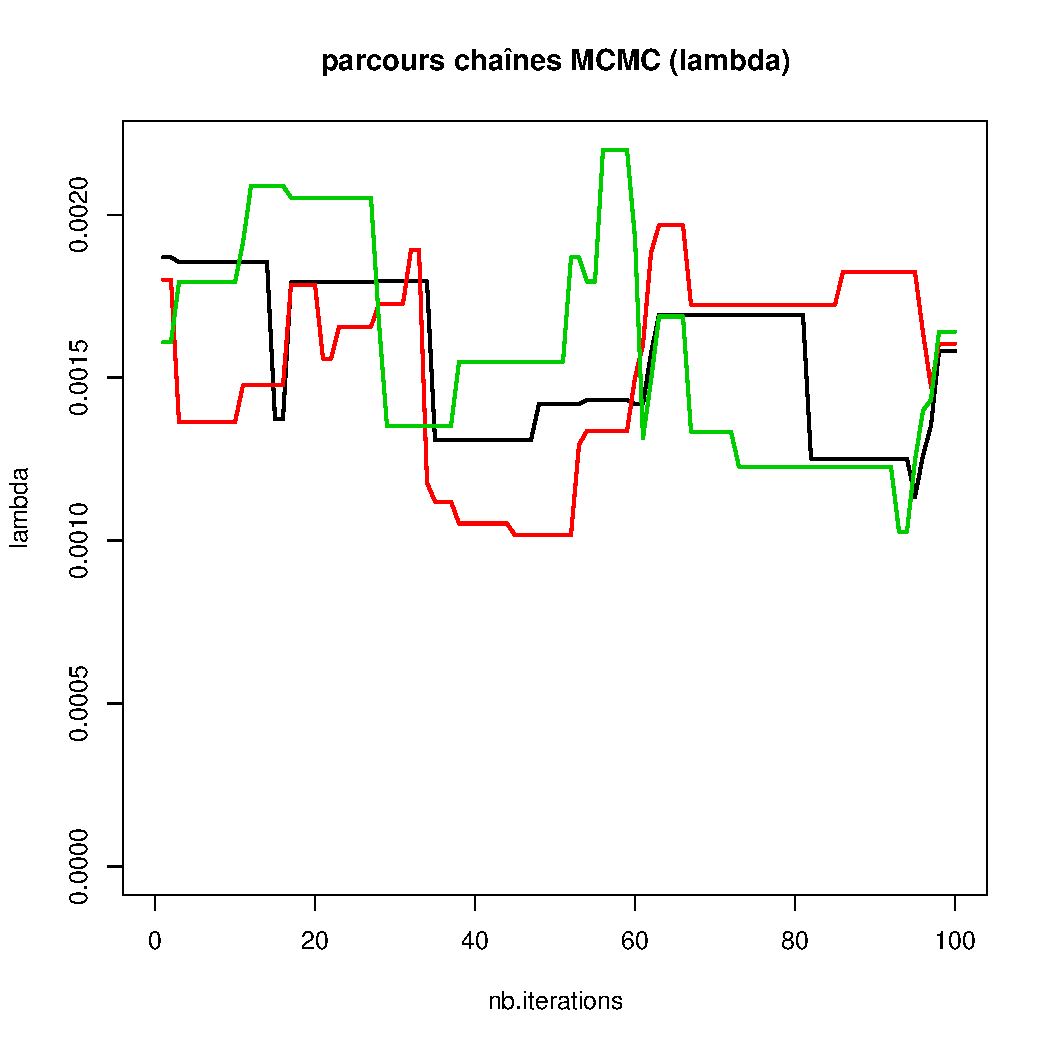
\includegraphics[width=6cm,height=5cm]{figures/calcul/MCMC1.pdf}
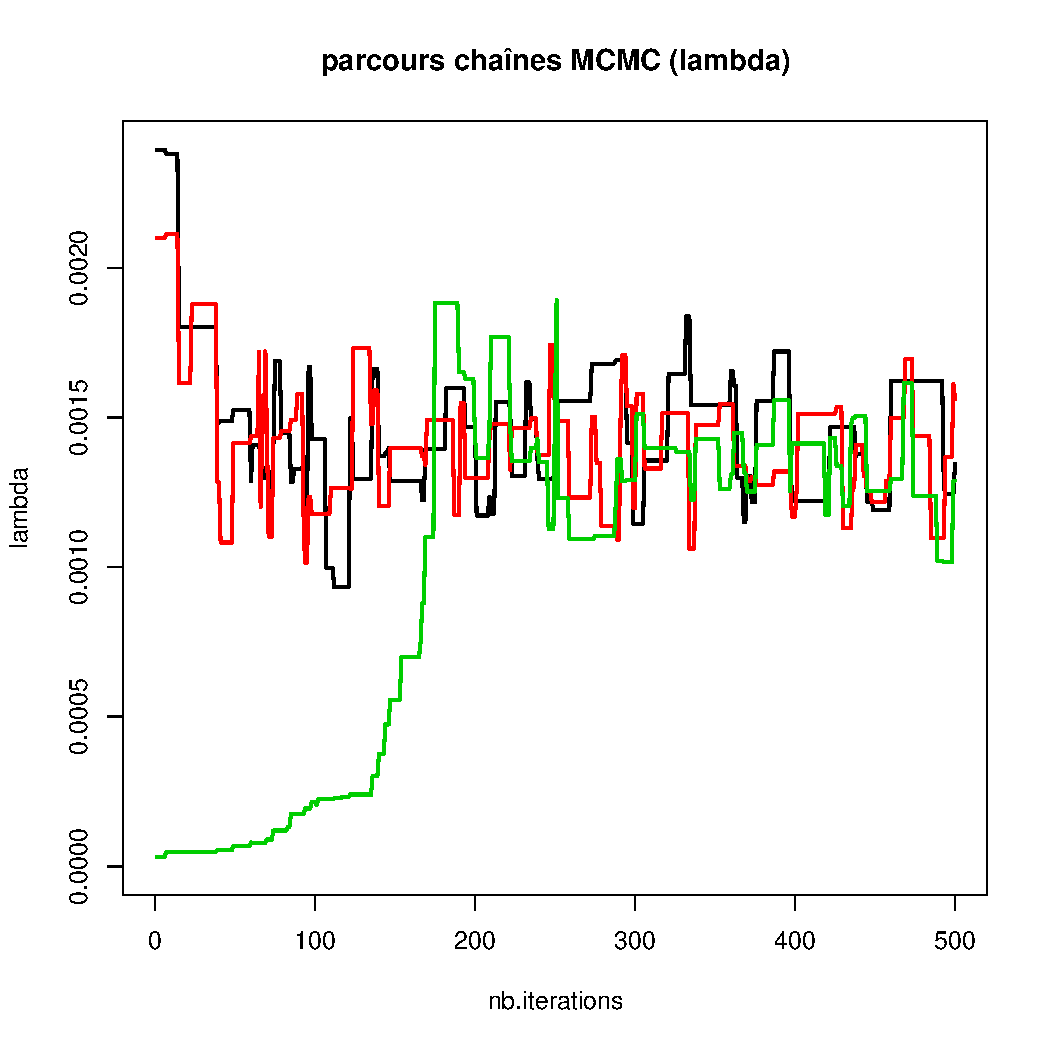
\includegraphics[width=6cm,height=5cm]{figures/calcul/MCMC2.pdf}
\end{center}
\end{rep}
\fi

\paragraph{Heuristique de progression du taux d'acception moyen $\alpha$.} Dans une chaîne MCMC produite par HM, la \emph{stationarité} est l'atteinte par une chaîne d'un tirage stationnaire dans la loi {\it a posteriori}. La rapidité de convergence vers la stationarité est induite par le taux d'acceptation $\alpha$. Au début de la MCMC, on cherche à \emph{explorer l'espace} : $\alpha$ grand ($\simeq 0.5$). Si $\alpha$ est petit, la simulation est fortement dépendante du passé de la chaîne : l'exploration de l'espace est très lente. Si $\alpha$ reste grand, chaque chaîne évolue solitairement et elles risque de se mélanger lentement. De différents travaux appliqués et théoriques, on a tiré une règle du pouce : un $\alpha=0.25$ est souvent considéré, en pratique (en particulier lorsque $\dim\Theta$ est grande) comme 
un bon objectif de renouvellement à la stationnarité. Par ailleurs, la calibration de $\rho(\theta|\theta^{(i-1)})$ (en général, le choix de sa variance) peut être en général faite de façon {\bf empirique} en ``testant" le taux d'acceptation effectif. \\

\paragraph{Heuristique de choix d'une loi instrumentale $\rho(\theta|...)$.} Dans le cas le plus simple, on choisit volontiers  $\rho(\theta|\theta^{(i-1)})=\rho(\theta)$ (\emph{loi statique}). Mais une modélisation standard est de choisir $\rho(\theta|\theta^{(i-1)})$ centrée sur $\theta^{(i-1)}$, et donc seule la variance doit être calibrée (ou le coefficient de variation). \\

\begin{exo}
Marche aléatoire $\theta \sim \theta^{(i-1)} +  \sigma \epsilon_i$ où $\epsilon_i \sim {\cal{N}}(0,1)$. \\
\end{exo}

\`A la différence du noyau, le caractère markovien de $\rho$ peut être relâché : on peut construire des $\rho$ {\bf adaptatives} en
utilisant tout le passé de la chaîne et non pas le dernier état connu $\theta^{(i-1)}$. Il existe une très vaste littérature à ce sujet, plutôt du domaine de la recherche que de la règle du pouce ou la ``boîte à outils". Là encore, on conseille de se référer à l'ouvrage \cite{Marin2007}. \\

\paragraph{Arrêt de chaîne MCMC.} Une fois que le \emph{temps de chauffe} est passée, la \emph{phase ergodique} est atteinte. De nombreux diagnostics de convergence vers la stationarité ont été proposés \cite{Cowles1996} et \emph{nécessitent d'avoir lancé plusieurs chaînes parallèles}. \`A la stationarité, ces chaînes parallèles se sont bien mélangées et ont ``oublié" le passé de chacune. Les diagnostics sont surtout \emph{visuels} : on regarde l'évolution du comportement d'une statistique informant sur la stabilité
de la distribution des $\theta$. \\

Parmi ces diagnostics de convergence, les statistiques de Gelman-Rubin (1992, cas 1D) et de Brooks-Gelman (1998, cas multidimensionnel) sont très standards : elles sont fondées sur la comparaison de variances inter et intra chaînes. \\

\begin{definition}{\bf Diagnostic de Gelman-Rubin.}
\begin{itemize}
\item Soit $P$ trajectoires (chaînes) parallèles de longueur $n$ (en pratique, $P = 3$.)
\item Soit $\theta^{(i)}_k$ la $i^{\text{ième}}$ réalisation sur la trajectoire $k$.
\item Soit $B$ l'estimateur de la \emph{variance de $\theta$ inter-chaînes}. 
\begin{eqnarray*}
B & = & \frac{n}{P-1}\sum\limits_{k=1}^P \left(\bar{\theta}_k - \bar{\theta}\right)^2
\end{eqnarray*}
avec
\begin{eqnarray*}
\bar{\theta}_k & = & \frac{1}{n}\sum\limits_{i=1}^n \theta^{(i)}_k \ \ \ \text{et} \ \ \ \bar{\theta} = \frac{1}{P} \sum\limits_{k=1}^P \bar{\theta}_k 
\end{eqnarray*}
\item soit $W$ l'estimateur de la \emph{variance de $\theta$ intra-chaînes} ({\bf ergodique})
\begin{eqnarray*}
W & = & \frac{1}{P}\sum\limits_{k=1}^P \left[\frac{1}{n-1}\sum\limits_{i=1}^n  \left({\theta}^{(i)}_k - \bar{\theta}_k\right)^2\right]
\end{eqnarray*}
\end{itemize}
Alors, { le rapport} (\emph{ statistique de Gelman-Rubin})
\begin{eqnarray*}
R & = & \frac{\frac{(n-1)}{n}W + \frac{1}{n}B}{W}
\end{eqnarray*}
{ tends vers 1 par valeurs supérieures}.
\end{definition}

En reprenant l'exemple \ref{debit.extreme}, on représente ci-dessous des exemples de trajectoires du taux d'acceptation et du  diagnostic de Brooks-Gelman, qui généralise Gelman-Rubin en tenant compte de la covariance entre dimensions d'une même chaîne. \\

\begin{center}
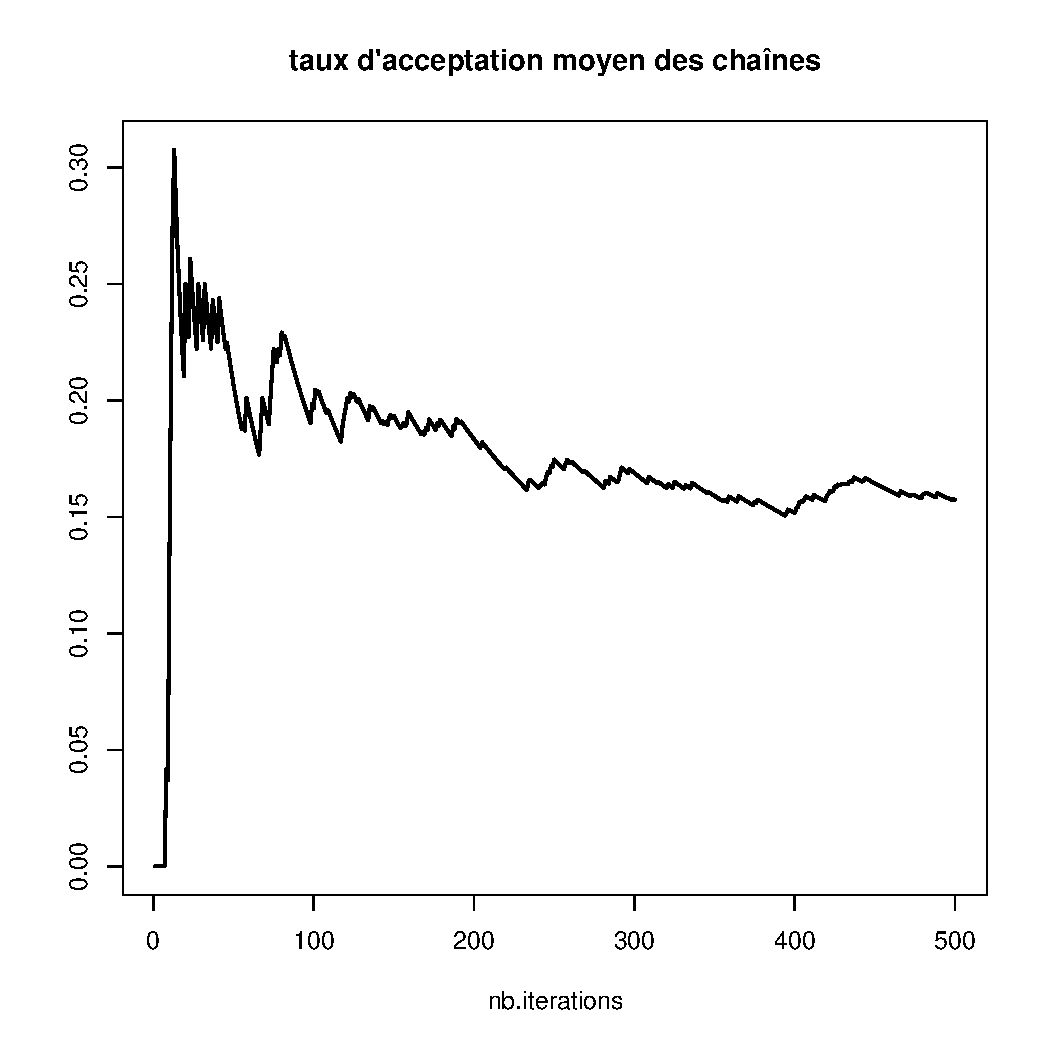
\includegraphics[width=7cm,height=7cm]{figures/calcul/alpha1.pdf}
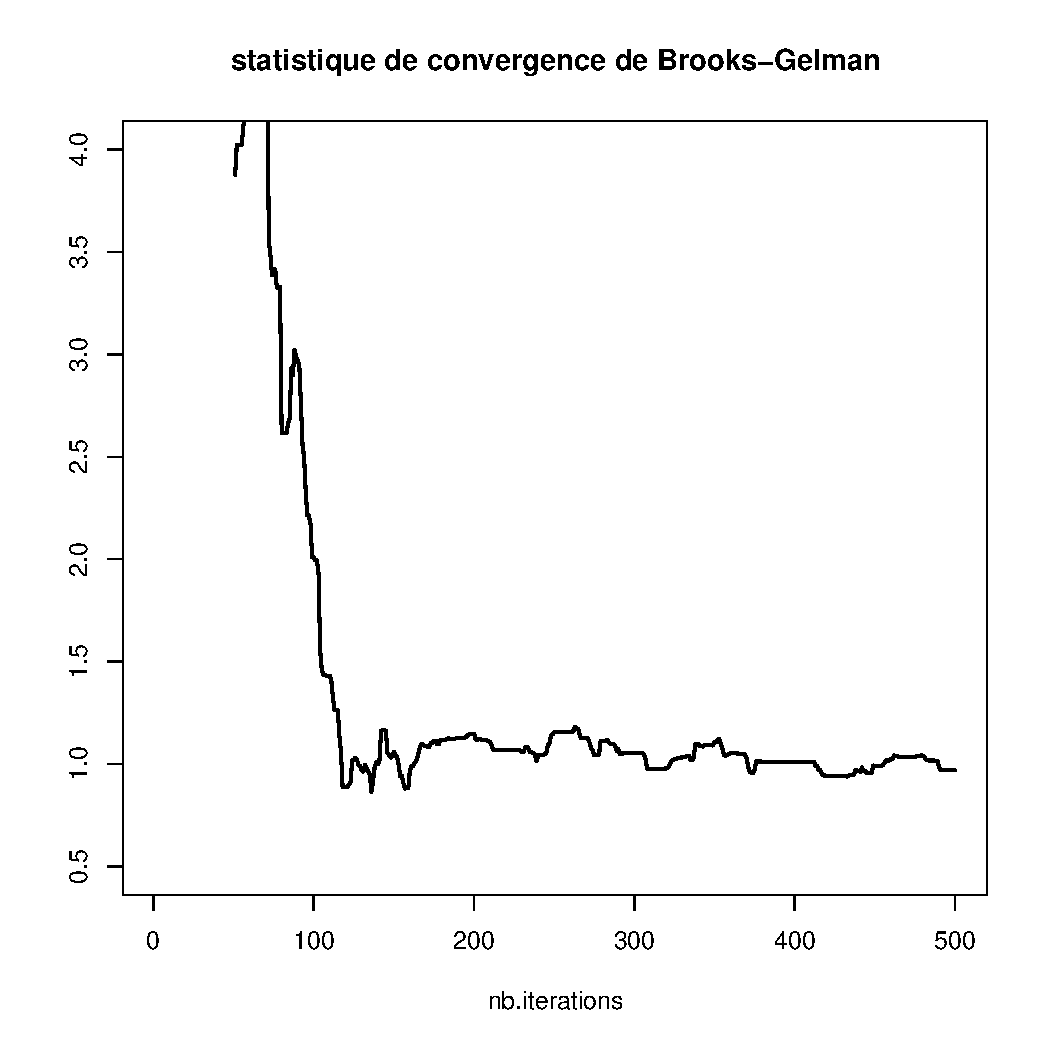
\includegraphics[width=7cm,height=7cm]{figures/calcul/bg1.pdf}
\end{center}

\paragraph{Décorrélation d'un échantillon MCMC.}
Soit $M_c$ le nombre d'itérations d'une MCMC avant qu'on atteigne la stationnarité (\textcolor{black}{\it temps de chauffe}, cf. figure \ref{ex-mcmc-1}). En sortie de la MCMC, on obtient un échantillon de $M-M_c$ vecteurs $\theta^{(M-M_c+1)},\ldots,\theta^M$
qui suivent la loi stationnaire $\pi(\theta|{\bf x_n})$. \\

\begin{figure}[!h]
\centering
\includegraphics[scale=0.45]{figures/calcul/mcmc-FR-1.jpeg}
\caption{Trois cha\^ines MCMC convergeant en parall\`ele vers la m\^eme loi-cible {\it a posteriori}. La p\'eriode de {\it chauffe} correspond au nombre d'it\'erations n\'ecessaire au m\'elange des cha\^ines, qui est un indicateur de l'atteinte de la stationnarit\'e. }
\label{ex-mcmc-1}
\end{figure} 


De par le caractère markovien de la MCMC, ces valeurs peuvent être \textcolor{black}{très dépendantes} le long d'une chaîne. Si on dispose de beaucoup de chaînes parallèles indépendantes, il suffit de prélever une valeur dans chacune... (mais c'est peu faisable en pratique). \\


 Pour obtenir un échantillon décorrélé (qui offre une meilleure information sur les caractéristiques de la loi $\pi(\theta|{\bf x_n})$), une bonne fa\c con de faire repose sur l'usage de l'\emph{autocorrélation}, de fa\c con similaire au traitement des \emph{séries temporelles}. \\
 
 On peut procéder comme suit :
 
 \begin{center}
 \begin{tabular}{|p{0.9\textwidth}|}
    \hline\\
    {{\bf Procédure de décorrélation.}
     \begin{enumerate}
\item On estime l'\textcolor{black}{autocorrélation} des éléments d'une chaîne:
\begin{eqnarray*}
\mbox{Aut}_{i,i+j} & = & \frac{\E\left[\left(\theta^{(i)} - \E[\theta|{\bf x_n}]\right)\left(\theta^{(i+j)} - \E[\theta|{\bf x_n}]\right)\right]}{\mbox{Var}[\theta|{\bf x_n}]}
\end{eqnarray*} 
à valeur dans $[-1,1]$. 

\begin{itemize}
%\item \scriptsize l'estimation empirique des quantités est faite en moyennant sur les chaînes parallèles
\item  \`A $i$ fixé, $\mbox{Aut}_{i,i+j}$ tends vers 0 lorsque $j$ augmente $\Leftrightarrow$ $\theta^{(i+j)}$ devient de plus en plus décorrélé de $\theta^{(i)}$. 
\item  On considère que cette décorrélation est effective lorsque l'estimateur de $\mbox{Aut}_{i,i+j}$ est un {\bf bruit blanc gaussien}.
\item  On peut donc, en moyenne sur les $i$, estimer le nombre d'itérations nécessaire $t$ pour obtenir 2 valeurs décorrélées de $\theta$.   
\end{itemize}


\item Sur chaque chaîne, on sélectionne le sous-échantillon ({\it thinning})
\begin{eqnarray*}
\theta^{(M-P+1)},\theta^{M-P+1+t},\theta^{M-P+1+2t},\ldots.
\end{eqnarray*}



\item On baisse encore la dépendance des éléments de l'échantillon final en prélevant dans les chaînes indépendantes. 
\end{enumerate}}  \\
\hline
    \end{tabular} 
    \end{center}
    \hspace{0.5cm}
    

\subsubsection{\'Echantillonneur de Gibbs et approches hybrides}

Dans un cas où  le param\`etre $\theta=(\theta_1,\ldots,\theta_d)$ est multidimensionnel (ce qui concerne notamment pour les mod\`eles hi\'erarchiques), il est recommand\'e d'utiliser une algorithmique d'{\it \'echantillonnage de Gibbs} \cite{Robert2004} qui tire parti du principe de \emph{cascade rule} ($\S$ \ref{multidim.sim}). \\

\'Etant donné un échantillon ${\bf x_n}$,  supposons disposer des lois {\it a posteriori} conditionnelles   
\begin{eqnarray*}
\theta_1|\theta_2,\ldots,\theta_d,{\bf x_n} & \sim & \pi(\theta_1|\theta_2,\ldots,\theta_d,{\bf x_n}), \\
\theta_2|\theta_1,\theta_3,\ldots,\theta_d,{\bf x_n} & \sim & \pi(\theta_2|\theta_1,\theta_3,\ldots,\theta_d,{\bf x_n}), \\
\ldots & & \ldots.
\end{eqnarray*} 
Alors la cha\^ine de Markov de vecteurs 
\begin{eqnarray*}
\theta^{(1)}=\left(\begin{array}{l} \theta^{(1)}_1 \\ \ldots \\ \theta^{(1)}_d\end{array}\right) \ , \hspace{0.5cm} \theta^{(i)}=\left(\begin{array}{l} \theta^{(M)}_1 \\ \ldots \\ \theta^{(M)}_d\end{array}\right) \ , \ldots
\end{eqnarray*}
produite par la simulation conditionnelle it\'er\'ee converge \'egalement vers la loi {\it a posteriori}-cible $\pi(\theta|{\bf x_n})$, sous des conditions tr\`es g\'en\'erales. \\

Lorsque les lois {\it a posteriori} conditionnelles ne sont elles-m\^emes pas compl\`etement explicites, une d\'emarche hybride, dite de {\it Metropolis-Hastings-within-Gibbs}, consiste \`a faire appel \`a un test de Metropolis pour chaque dimension.

\begin{remark} 
La solution proposée pour l'exercice \ref{debit.extreme} est d'ailleurs un exemple d'algorithme de Gibbs en dimension 2, incluant une étape de Metropolis-Hastings pour l'estimation du paramètre $\lambda$. 
\end{remark}

L'algorithmique de Gibbs (hybride), qui exploite au maximum la structure conditionnelle des modèles hiérarchiques, est donc très générale, et elle est notamment particulièrement intéressante lorsqu'on traite des \emph{problèmes à données manquantes} (ex : présentant des données censurées, ou des variables latentes comme les modèles de mélange...). Dans un cadre bayésien, il permet de considérer ces données comme des paramètres inconnus à simuler {\it ({augmentation de données})}. L'exemple suivant illustre ce procédé. 

\begin{exec}{\bf (Retour à l'exercice \ref{quasi.conjug}).}. 
 On suppose de nouveau connaître un échantillon ${\bf x_n} \sim {\cal{N}}(\theta,1)$ composé de quelques observations $x_1,\ldots,x_{n-1}$ supposées iid de loi ${\cal{N}}(\theta,1)$, et d'une  pseudo-observation $y$ qui est un cas-limite masquant ({\it censurant}) une observation $x_{n}$ qui aurait dû être faite: $y<x_{n}$. On considère toujours $\theta \sim {\cal{N}}(\mu,1)$ {\it a priori}. 
Pouvez-vous produire un algorithme d'échantillonnage par Gibbs qui génère des réalisations de la loi {\it a posteriori} de $\theta$ ? 
\end{exec}

\if\mycmdexotwo1 \vspace{1cm} \begin{rep}
Si on connaissait $x_n$, le modèle bayésien serait conjugué et
\begin{eqnarray*}
\theta|{\bf x_n} & \sim & {\cal{N}}\left(\frac{1}{n}\left(\mu + \sum\limits_{i=1}^n x_i\right),(n+1)^{-1}\right)
\end{eqnarray*}
 On considère alors la donnée manquante $x_{n}$ comme un paramètre inconnu et aléatoire.  Sachant $\theta$ et ${\bf x_n}$, on peut montrer par la règle de Bayes que la loi de la variable aléatoire manquante $X_n$ est la normale tronquée
\begin{eqnarray*}
{\cal{N}}(\theta,1)\cdot \1_{\{x_n\geq y\}}.
\end{eqnarray*}
En effet, la fonction de répartition de $X_n$ est conditionnelle : $P(X_n<x|X_n>y)$. Par la règle de Bayes
\begin{eqnarray*}
P(X_n<x|X_n>y) & = & \frac{P(X_n<x \cap X_n>y)}{P(X_n>y)} \ = \ \frac{P(y<X_n<x)}{P(X_n>y)}.
\end{eqnarray*}
Le dénominateur est une constante (indépendante de $x$). Donc
\begin{eqnarray*}
P(X_n<x|X_n>y) & \propto & \int_{y}^x f_X(u) \ du \ = \ \int_{-\infty}^x f_X(u) \1_{\{y\leq u\}} \ du
\end{eqnarray*}
où $f_X$ est la densité d'un $X$ non-contraint (ici gaussienne). On en déduit que la densité de $X_n$ est
\begin{eqnarray*}
f_{X_n}(x) & = & \frac{f(x)\1_{\{y\leq x\}}}{\int_{-\infty}^{\infty} f(u)\1_{\{y\leq u\}} \ du}.
\end{eqnarray*}

L'algorithme de Gibbs à mettre en oeuvre est donc le suivant :
\texttt{
\begin{itemize}
\item On part d'une valeur $\theta^{(0)}$
\item Itération $i\geq 1$ :
\begin{enumerate}
\item on simule $x^{(i)}_{n} \sim {\cal{N}}\left(\theta^{(i-1)},1\right)\cdot \1_{\{x_n\geq y\}}$
\item on simule $\theta^{(i)} \sim  {\cal{N}}\left(\frac{1}{n}\left(\mu + \sum\limits_{i=1}^{n-1} x_i + x^{(i)}_{n}\right),(n+1)^{-1}\right)$
\end{enumerate}
\end{itemize}
}

\end{rep}



\fi
\vspace{0.5cm}

La modélisation bayésienne par conditionnement peut fréquemment entra\^iner le mécanisme suivant : 
\begin{enumerate}
\item On construit un {\it a priori} \emph{hiérarchique}
\begin{eqnarray*}
\pi(\theta) & = & \pi(\theta_1|\theta_2,\theta_3)\pi(\theta_2|\theta_3)\pi(\theta_3)
\end{eqnarray*}
avec des {\it a priori} non-informatifs
\item Ce conditionnement est souvent choisit pour tirer parti de \emph{conjugaisons} {\it a posteriori} : les lois conditionnelles
\begin{eqnarray*}
\pi(\theta_1|{\bf x_n},\theta_2,\theta_3), \\
\pi(\theta_2|{\bf x_n},\theta_1,\theta_3), \\
\pi(\theta_3|{\bf x_n},\theta_1,\theta_2)
\end{eqnarray*}
sont explicites, ce qui permet d'utiliser un algorithme de Gibbs.
\end{enumerate}
Toutefois,  même si ces lois {\it a posteriori} \emph{conditionnelles}  sont propres, la loi \emph{jointe} peut ne pas l'être :
\begin{eqnarray*}
\int_{\Theta} \pi(\theta|{\bf x_n}) \ d\theta & = & \infty.
\end{eqnarray*}
Il est donc indispensable de vérifier la \emph{propriété} {\it a posteriori} avant de mettre en oeuvre un algorithme de Gibbs. 



\begin{exec}{\bf Modèle à effets aléatoires autour d'une constante  (Hobert-Casella).}
Pour $i=1,\ldots,I$ et $j=1,\ldots,J$, on considère 
\begin{eqnarray*}
x_{ij} &  = & \beta + u_i + \epsilon_{ij}
\end{eqnarray*}
où $u_i\sim {\cal{N}}(0,\sigma^2)$ et $\epsilon_{ij}\sim {\cal{N}}(0,\tau^2)$. Ce type de modèle permet de représenter la distribution d'une caractéristique au sein d'une population, où  $\beta$ est une tendance moyenne, $u_i$ correspond à une  variation d'un groupe et $\epsilon_{ij}$ à une  variation au sein d'un sous-groupe. On suppose choisir 
\begin{eqnarray*}
\pi(\beta,\sigma^2,\tau^2) & \propto & \frac{1}{\sigma^2\tau^2} \ \ \ \text{(prior de Jeffreys)}.
\end{eqnarray*}
On note ${\bf x_{IJ}}$ l'échantillon des données observées, $\bar{x}_i$ la moyenne sur les $j$. On note ${\bf u_I}$ l'échantillon manquant des $u_1,\ldots,u_I$ (reconstitué dans l'inférence). 
\begin{enumerate}
    \item Calculer les lois conditionnelles {\it a posteriori} de 
\begin{eqnarray*}
U_i|{\bf x_{IJ}},\beta,\sigma^2,\tau^2 &  &  \\
\beta|{\bf x_{IJ}},\sigma^2,\tau^2,{\bf u_I} &  &  \\
\sigma^2|{\bf x_{IJ}},\beta,\tau^2,{\bf u_I} &  &  \\
\tau^2|{\bf x_{IJ}},\beta,\sigma^2,{\bf u_I} & & 
\end{eqnarray*}
Ces lois sont-elles bien définies ?
\item Donner une formule (à un coefficient proportionnel près) pour la loi {\it a posteriori} jointe $\pi(\sigma^2,\tau^2|{\bf x_{IJ}})$. Comment se comporte-t-telle au voisinage de $\sigma=0$, pour $\tau\neq 0$ ? Que pouvez-vous en déduire ? 
\item Mettre en place un algorithme de Gibbs permettant d'inférer sur $(\beta,\sigma^2,\tau^2)$. 
Que pouvez-vous dire sur la convergence des chaînes MCMC ?
\end{enumerate}
\end{exec}

\if\mycmdexotwo1 \vspace{1cm} \begin{rep}
\begin{enumerate}
\item Des calculs algébriques montrent que les lois conditionnelles sont
\begin{eqnarray*}
U_i|{\bf x_{IJ}},\beta,\sigma^2,\tau^2 & \sim & {\cal{N}}\left(\frac{J(\bar{x}_i-\beta)}{J+\tau^2\sigma^{-2}},(J\tau^{-2} + \sigma^{-2})^{-1}\right) \\
\beta|{\bf x_{IJ}},\sigma^2,\tau^2,{\bf u_I} & \sim & {\cal{N}}\left(\bar{x}-\bar{u},\tau^2/IJ\right) \\
\sigma^2|{\bf x_{IJ}},\beta,\tau^2,{\bf u_I} & \sim &  {\cal{IG}}\left(I/2,(1/2)\sum\limits_{i=1}^I u^2_i\right) \ \ \ \ \ \text{\it (loi inverse gamma)} \\
\tau^2|{\bf x_{IJ}},\beta,\sigma^2,{\bf u_I} & \sim &  {\cal{IG}}\left(IJ/2,(1/2)\sum\limits_{i=1}^I\sum\limits_{j=1}^J (x_{ij} - u_i - \beta)^2\right)  
\end{eqnarray*}
qui sont donc bien définies. 
\item La loi {\it a posteriori} jointe 
\begin{eqnarray*}
\pi(\sigma^2,\tau^2|{\bf x_{IJ}}) & = & \int \pi(\beta,\sigma^2,\tau^2|{\bf x_{IJ}}) \ d\beta \\
                                  & = & \int\left[\int_1\ldots\int_i\ldots\int_I \pi(\beta,\sigma^2,\tau^2|{\bf x_{IJ}}) \ d u_i\right] d\beta \\
\end{eqnarray*}
est proportionnelle à
\begin{eqnarray*}
\frac{\sigma^{-2-I}\tau^{-2-IJ}}{\left(J\tau^{-2} + \sigma^{-2}\right)^{I/2}}\sqrt{\tau^2 + J\sigma^2} \exp\left\{-\frac{1}{2\tau^2}\sum\limits_{i,j} (y_{ij}-\bar{y}_i)^2 - \frac{J}{2'\tau^2 + J\sigma^2)}\sum\limits_{i} (\bar{y}_i-\bar{y})^2\right\}
\end{eqnarray*}
qui se comporte comme $\sigma^{-2}$ au voisinage de $\sigma=0$, pour $\tau\neq 0$. Cette loi jointe n'est donc pas intégrable ({\it propre}). 
\item On constate normalement une absence de convergence claire des chaînes, ou une stationnarité (momentanée) trompeuse.
\end{enumerate}
\end{rep}
\fi
\vspace{0.5cm}

\clearpage

\subsubsection{Un résumé de ces premières méthodes}

On trouvera sur le tableau ci-dessous quelques informations qui résument l'usage et les particularités de ces algorithmes de calcul bayésien. Pour aider à faire un choix, voici quelques conseils reposant sur quelques questions essentielles.
\begin{itemize}
\item La loi-cible {\it a posteriori} est-elle proche d'un cas explicite (ou conjuguée) (ex: loi normale censurée) ?
\item Si oui, que faudrait-il faire (typiquement, \emph{simuler des données manquantes} $\Rightarrow$ Gibbs)
\item En multidimensionnel, a-t-on des propriétés de conjugaison conditionnelles ($\Rightarrow$ Gibbs) ? 
\item Si nous n'avons aucune idée, peut-on trouver une loi $\rho(\theta)$ partageant certaines caractéristiques avec $\pi(\theta|{\bf x_n})$ ?
\begin{itemize}
\item Par exemple, on peut tenter de tracer  $\pi(\theta|{\bf x_n})$ (à un coefficient près) dans les cas unidimensionnels. 
\item On peut également mener un calcul du  mode {\it a posteriori} $\hat{\theta}$ = maximum de la vraisemblance pondérée par l'{\it a priori}.
\item une idée de loi instrumentale typique est ainsi une loi $\rho(\theta)$  gaussienne ${\cal{N}}(\hat{\theta},\sigma^2I_d)$ avec $\sigma$ calibré empiriquement. 
\end{itemize}
\end{itemize}


\begin{tabular}{l|l|l|l|l}
          & \textcolor{purple}{Acceptation -} & \textcolor{purple}{\'Echant.} & \textcolor{purple}{Métropolis -} & \textcolor{purple}{Gibbs}  \\
          & \textcolor{purple}{Rejet}         & \textcolor{purple}{d'importance} & \textcolor{purple}{Hastings (MH)}  &  \\
\hline
\emph{Contexte}  & &&& \\
\cline{1-1}
Dimension de $\theta$ & 1 & grande & grande & grande \\
Nature simulation  & iid  & non-indep.$^*$ & non-indep. approx.$^*$ & non-indep. approx.$^*$ \\
Nature algo & itératif          & statique   & itératif & itératif \\ 
& &&& \\
\emph{Nb. itérations typ.} & quelques       & 1 & quelques dizaines  & quelques \\
                                      & centaines      &   & de milliers        & milliers \\
& &&& \\
\emph{Implémentation} & aisée & aisée & calibration fine & aisée \\
                                 &       &       & de $\rho(\theta)$  nécessaire & \\
& &&& \\
\emph{Critère d'arrêt} & aucun & aucun   & nécessaire   & nécessaire \\
& &&& \\
\textcolor{red}{Risques} & fort taux  & poids mal   & mauvais mélange   & nécessite souvent \\
            & de rejet                     &  équilibrés           &   chaînes //                       & couplage avec M-H \\
& &&& \\
\textcolor{red}{Temps de calcul} & long & rapide & long & plut\^ot rapide \\
\hline
\end{tabular}

%%%%%%%%%%%%%%%%%%%%%%%%%%%%%%%%%%%%%%
\clearpage
\subsection{Méthodes d'échantillonnage accélérées}

Les méthodes MCMC ont été et restent très utilisées pour simuler des valeurs {\it a posteriori} $\theta_1,\ldots,\theta_n \overset{iid}{\sim} \pi(\theta|x)\propto f(x|\theta)\pi(\theta)$. Elles sont toutefois lentes pour des problèmes complexes, et la convergence vers la loi-limite ({\it a posteriori} dans un cadre bayésien) reste difficile à vérifier. En particulier, les \emph{méthodes MCMC restent très lourdes} (voire impossibles) à utiliser dans les problèmes de type ``Big Data". \\

\begin{exo}
Modèles à états latents, tels les modèles de Markov cachés permettant de segmenter des images structurées de fa\c con non supervisée... \\
\end{exo}

Ainsi, des avancées importantes pour {\bf accélérer les algorithmes d'échantillonnage} ont été menées :
\begin{itemize}
\item en se fondant sur des techniques de \emph{réduction de variance} ; 
\item en démarrant les chaînes de Markov \emph{au plus proche du mode {\it a posteriori}}  ; 
\item en \emph{améliorant le choix des lois instrumentales}, inspirées par la physique énergétique (dynamique, particules, quantique...).
\end{itemize}
Nous en listons ci-dessous quelques-unes. \\

\noindent Soulignons cependant que dans un cadre d'usage de plus en plus soumis aux contraintes de grande dimensionalité et d'apprentissage massif, dans la réalité des faits, on calcule rarement la distribution {\it posteriori}. On préfère se simplifier la vie et les calculs en approximant la loi distribution {\it posteriori} par une valeur unique (\texcolor{black}{mode a posteriori}). Il s'agit ni plus ni moins d'une \emph{maximisation de vraisemblance pénalisée} (voir $\S$ \ref{estimation.MAP.ML} pour plus de détails). Dans ce contexte, les les \emph{techniques d'optimisation}, comme l'algorithme EM ou le Gradient Boosting,  ont encore de beaux jours devant elle, et il est possible d'interpréter ces algorithmes comme des approches "dégénératives" du cadre MCMC.   


\subsubsection{Réduction de variance par utilisation des corrélations négatives (variables antithétiques)}

Considérons deux échantillons iid $(\theta_1,\ldots,\theta_m)$ et $(\tilde{\theta}_1,\ldots,\tilde{\theta}_m)$ suivant $\pi(\theta|D)$ pour estimer
$$
{\cal{H}} = \int_{\R} h(\theta) \pi(\theta|D) \ d\theta.
$$
Soient
$$
\hat{\cal{H}}_1 = \frac{1}{m} \sum\limits_{i=1}^m h(\theta_i)  \ \ \  \ \text{et} \ \ \ \ \hat{\cal{H}}_2 = \frac{1}{m} \sum\limits_{i=1}^m h(\tilde{\theta}_i)
$$
de moyenne $m$ et de variance $\sigma^2$. Alors, la variance de la moyenne vaut
$$
\V\left[\frac{1}{2}\left(\hat{\cal{H}}_1+ \hat{\cal{H}}_2\right) \right]  = \frac{\sigma^2}{2} + \frac{1}{2} \mbox{Cov}\left(\hat{\cal{H}}_1,\hat{\cal{H}}_2 \right)
$$
Par conséquent, si les deux échantillons sont \emph{négativement corrélés}, 
$$
\mbox{Cov}\left(\hat{\cal{H}}_1,\hat{\cal{H}}_2 \right) \leq 0
$$
ils font mieux que deux échantillons de même taille. Ce type d'approche a été formalisé sous le nom de \emph{réduction de variance par variables antithétiques} :
\begin{enumerate}
\item Si $\pi(\theta|D)$ symétrique autour de $\mu$, prendre $\tide{\theta}_i = 2\mu- \theta_i$ ; 
\item Si $\theta_i = F^{-1}(U_i)$, prendre $Y_i = F^{-1}(1-U_i)$ ; 
\item Si $(A_i)_i$ est une partition de $\Theta$, produire un échantillonnage \emph{partitionné} (ou  \emph{stratifié}) en choisissant des $\theta_j$ dans chaque $A_i$ (nécessite de connaître $\Pi(A_i)$).
\end{enumerate}


\subsubsection{Variables de contrôle}

Soit
$$
{\cal{H}} = \int_{\R} h(\theta) \pi(\theta|D) \ d\theta
$$
à évaluer et 
$$
{\cal{H}}_0 = \int_{\R} h_0(\theta) \pi(\theta|D) \ d\theta
$$
connue. On estime quand même ${\cal{H}}_0$ par $\hat{\cal{H}}_0$ (et ${\cal{H}}$ par $\hat{\cal{H}}$). Dans ce cas, on peut définir un {\bf estimateur combiné} :
$$
\hat{\cal{H}}^* =  \hat{\cal{H}} + \beta\left(\hat{\cal{H}}_0-{\cal{H}}_0\right)
$$

\begin{proposition}
$\hat{\cal{H}}^*$ est sans biais pour ${\cal{H}}$ et 
$$
\V\left[\hat{\cal{H}}^* \right] = \V\left[\hat{\cal{H}} \right] + \beta^2  \V\left[\hat{\cal{H}}_0 \right] + 2\beta \mbox{Cov}\left(\hat{\cal{H}} ,\hat{\cal{H}}_0 \right).$$
\end{proposition}

On peut alors faire un choix optimal de $\beta$, qui permet de diminuer la variance de l'estimateur :
$$
 \beta^* = - \frac{\mbox{Cov} \left(\hat{\cal{H}} ,\hat{\cal{H}}_0 \right)}{\V\left[\hat{\cal{H}}_0 \right]} 
$$
avec  
$$
\V\left[\hat{\cal{H}}^* \right] =  \V\left[\hat{\cal{H}} \right] \left(1-\rho^2\right)
$$
où $\rho^2$ est le coefficient de corrélation entre $\hat{\cal{H}}$ et $\hat{\cal{H}}_0$. \\

\begin{exo}{\bf Approximation de quantile.}
Supposons vouloir évaluer 
$$
q = \Pi(\theta>a|D) \ = \ \int_a^{\infty} \pi(\theta|D) \ d\theta
$$
par
$$
\hat{q} = \frac{1}{n} \sum\limits_{i=1}^n \1_{\{\theta_i > a\}}, \ \ \ \ \ \theta_i \overset{iid}{\sim} \pi(\theta|D)
$$
avec
$
\Pi(\theta>\mu|D) = 1/2
$. La variable de contrôle
$$
\frac{1}{n} \sum\limits_{i=1}^n \1_{\{\theta_i > a\}} + \beta\left(\frac{1}{n} \sum\limits_{i=1}^n \1_{\{\theta_i > \mu\}} - \Pi(\theta>\mu|D)\right)
$$
améliore $\hat{q}$ si
$$
\beta < 0 \ \ \ \ \text{et} \ \ \ \ |\beta|<2\frac{\Pi(\theta>a|D)}{\Pi(\theta>\mu|D)}.
$$


\end{exo}


\subsubsection{Rao-Blackwellisation}

On peut également vouloir tirer parti de l'inégalité 
$$
\V\left[\E[h(\theta)|Y]\right] \leq \V\left[h(\theta)\right],
$$
aussi appelée \emph{Théorème de Rao-Blackwell}, pour diminuer la variance d'un estimateur de Monte Carlo. 

\begin{proposition}
Si $\hat{\cal{H}}$ est un estimateur sans biais de ${\cal{H}}=\E_{\pi}\left[h(\theta)\right]$, avec $\theta$ simulé à partir de la densité jointe $\tilde{\pi}(\theta,y)$ où
$$
\int \tilde{\pi}(\theta,y) \ dy = \pi(\theta)
$$
alors l'estimateur
$$
\hat{\cal{H}}^* = \E_{\tilde{\pi}}\left[\hat{\cal{H}}|Y_1,\ldots,Y_n \right] 
$$
domine $\hat{\cal{H}}(\theta_1,\ldots,\theta_n)$ en variance (et est aussi sans biais).
\end{proposition}

L'algorithme EM, notamment, tire parti de ce procédé pour maximiser une vraisemblance de données incluant des données manquantes. 



%%%%%%%%%%%%%%%%%%%%%%%%%%%%%%%%%%%%%%
\subsubsection{Amélioration de lois instrumentales par dynamique de Langevin / hamiltonienne}

Les améliorations de lois instrumentales au sein des algorithmes de type MCMC sont généralement fondées sur des parallèles avec des problèmes de \emph{diffusion} / \emph{mouvement de système physique}  (particulaire), régis par des équations aux dérivées partielles (EDP). L'idée générale est d'utiliser de l'information sur la densité cible au travers du passé de l'algorithme, et plus précisément l'information contenue dans le \emph{gradient $\nabla \log \pi(\theta|D)$}. Le cadre général de la dynamique particulaire de Langevin offre une formalisation de ce problème. Par la suite, pour simplifier les notations, on notera $D$ les données disponibles. \\

\begin{proposition}{\bf Metropolis-Adjusted Langevin Algorithm (MALA)}
Discrétisation d'une diffusion de Langevin de probabilité stationnaire $\pi(\theta|D)$ :
\begin{eqnarray*}
\rho(\theta,.) & = & {\cal{N}}_d\left(\theta + \frac{h^2}{2}\nabla \log \pi(\theta|D), h^2 I_d\right)
\end{eqnarray*}
pour un pas $h>0$. Le choix de $h$ relève de considérations sur la structure de $\mbox{Cov}(\theta|D)$.
\end{proposition}

De fa\c con plus explicite, on veut simuler selon une loi non normalisée définie en termes de potentiel
$$
\pi(\theta|D)  \propto  \exp\left(-U(\theta)\right).
$$
Sous des conditions peu contraignantes, cette densité est l'unique mesure de probabilité invariante d'une \emph{équation différentielle stochastique de Langevin}
$$
\mbox{d}\theta_t  =  -\nablaU(\theta_t) \mbox{d}t + \sqrt{2}\mbox{d} B_t
$$
avec $B_t$ un processus brownien (qui décrit le mouvement d'une particule soumise à une infinité de chocs en des temps très courts)
$$
B_t \sim {\cal{N}}(0,t). 
$$
 En général on ne peut résoudre exactement l'équation précédente : on s'appuie alors sur l'approximation produite par une discrétisation d'Euler-Maruyama
$$
\theta_{k+1} = \theta_k - \gamma\nabla U(\theta_k) +  \sqrt{2\gamma} Z_{k+1}.
$$
Cette approche est l'\emph{Unadjusted Langevin Algorithm} (ULA) et s'appelle aussi \emph{Langevin Monte Carlo} (LMC). Il s'agit simplement d'un calcul de MAP par un algorithme de descente de gradient avec du bruit ajouté à chaque itération.
Des résultats théoriques ont été obtenus récemment pour contrôler l'erreur d'approximation / taille d'échantillon et dimension (si $\pi(\theta|D)$ régulière),par Dumus et Moulines (2017). Cette approche marche bien pour le traitement de la grande dimension de $\theta$ en inférence bayésienne. \\

Toutefois, cette discrétisation induit du biais, qui peut être ôté par une étape d'acceptation-rejet de Metropolis-Hastings, ce qui donne la formulation MALA de l'algorithme. L'algorithmique MALA hérite donc des bonnes propriétés de convergence de ULA et affronte bien la grande dimension. Dans un tour d'horizon récent, Nemeth et Fearnhead (2019) ont récemment montré que le pas optimal pour MALA est grand, mais MALA coûte plus cher par itération que les approches ULA. Par ailleurs, les lois instrumentales fondées sur ULA ont un meilleur taux d'acceptation que les marches aléatoires MALA. \\

\paragraph{Approche MYULA.} Quand $\pi(\theta|D)$ n'est pas régulière, on suppose que le potentiel peut s'écrire
$$
U(\theta) = f(\theta) + g(\theta)
$$
où $f$ est convexe, continûment différentiable, et de gradient lipschitzien ; $g$ est propre, convexe, et semi-continue à gauche. On peut alors remplacer $g$ par son enveloppe dite de Moreau-Yosida (voir figure \ref{MY}) :
\begin{eqnarray*}
g^{\lambda}(x) & = & \min\limits_{y\in \R^d} \left\{ g(y) + (2\lambda)^{-1} \|x-y\l^2\right\} \\
\nabla g^{\lambda}(x) & = & \lambda^{-1} \left(x-\mbox{prox}^{\lambda}_g(x)\right)
\end{eqnarray*}
avec
$$
\mbox{prox}^{\lambda}_g(x) = \arg\min\limits_{y\in \R^d} \left\{ g(y) + (2\lambda)^{-1} \|x-y\l^2\right\}. 
$$
L'algorithme de \emph{Moreau-Yosida ULA} (MYULA) s'écrit alors
$$
\theta_{k+1} = \left(1-\frac{\gamma}{\lambda}\right)\theta_k - \gamma\nabla f(\theta_k) + \frac{\gamma}{\lambda}\mbox{prox}^{\lambda}_g(\theta_k) + \sqrt{2\gamma} Z_{k+1}.
$$

\begin{figure}[hbtp]
\centering
\includegraphics[scale=0.4]{figures/calcul/unif11.png} 
\caption{Illustration issue de Nemeth et Fearnhead (2019).}
\label{MY}
\end{figure}

En général, avec $\pi(\theta|D) \propto \pi(\theta) \prod\limits_{i=1}^n f(x_i | \theta)$, on a
$$
U  = \sum\limits_{i=0}^n U_i
$$
avec $U_0(\theta)=-\log \pi(\theta)$ et $U_i(\theta) = -\log f(x_i | \theta)$. Le problème posé par cet algorithme est qu'une seule itération reste coûteuse.  L'idée est d'utiliser des approches de \emph{descente de gradient stochastique} (SGD) pour accélérer le calcul. \\

\paragraph{Descente de gradient stochastique (SGD).} La version "Langevin" du SGD ({\it Stochastic Gradient Langevin Dynamics}, ou SGLD) s'écrit simplement 
$$
\theta_{k+1} = \theta_k -  \gamma\left(\nabla U_0(\theta_k) + \frac{n}{p}\sum\limits_{i\in S_{k+1}}\nabla U_i(\theta_k)\right)  + \sqrt{2\gamma} Z_{k+1}.
$$
Cette approche obtient un très faible coût de calcul par itération si $p\ll n$. Il s'agit donc, en résumé, d'un calcul de MAP par un algorithme de descente de gradient avec du bruit ajouté à chaque itération, à l'image de ce qui est massivement utilisé en apprentissage statistique. Des résultats théoriques prouvant la bonne convergence de ce type d'algorithme ont été obtenus récemment par Brosse {\it et al.} (2018). \\

\paragraph{Autres variantes.} On peut hybrider le SGLD avec une approche par \emph{variables de contrôle} si on peut estimer  le mode  de $\pi(\theta|D)$. De telles approches se nomment \emph{SGLD Control Variate} (SGLDCV) ou \emph{SGLD Fixed Point} (SGLDFP). Elles nécessitent très souvent de lancer un premier SGLD pour estimer le mode, puis opèrent un raffinement. D'autres approches s'hybridant avec des techniques d'échantillonnage d'importance (ou stratifié, par exemple) existent également.  


\paragraph{Méthodes de Monte Carlo Hamiltoniennes (HMC).}
Les méthodes HMC, disponibles sous Python 3 (\texttt{PyMC}\footnote{\url{https://colcarroll.github.io/hamiltonian_monte_carlo_talk/bayes_talk.html}}) ou \texttt{STAN}\footnote{\url{https://mc-stan.org}}, sont des méthodes MCMC issues d'un parallèle entre deux problèmes :
\begin{itemize} 
\item produire une dynamique pour la chaîne de Markov $\theta_i,\ldots,\theta_j$ s'approchant de la loi visée $\pi(\theta|{\bf x_n})$ ;
\item prévoir le mouvement d'un système physique  soumis à une \emph{dynamique hamiltonienne}.
\end{itemize}
La dynamique hamiltonienne est une reformulation de la mécanique newtonienne selon laquelle la description d'un système est faite au travers de \emph{coordonnées} (généralisées) et de \emph{momentum} (quantité de mouvement), reliées par un {\bf lagrangien} ; celui-ci exprime une différence entre énergie cinétique et énergie potentielle. Le lagrangien est une fonction des variables dynamiques qui permet d'écrire les équations de mouvement. La transformée de Legendre de ce lagrangien est nommé \emph{hamiltonien}. Le tableau ci-dessous résume la correspondance algébrique entre les deux problèmes mentionnés :

\begin{center}
\begin{tabular}{l|l}
\hline
Système physique & Applications MCMC \\
\hline
Position & $\theta$ \\
\'Energie potentielle & $ -\log \pi(\theta|D)$ \\
Momentum & Variables introduites artificiellement \\
& (variables gaussiennes en général) \\
\hline
\end{tabular}
\end{center}

L'idée générale de l'application aux MCMC est la suivante : à chaque pas de la MCMC, on met à jour les momentum et on produit une nouvelle trajectoire-candidate pour $\theta$ (et non un simple tirage) suivant une dynamique hamiltonienne (approche {\it leapfrog}). \\

Un récapitulatif rapide des méthodes fondées sur un parallèle avec des modèles de  dynamique est présenté dans le résumé ci-dessous : \\

%\begin{figure}[hbtp]
\begin{center}
\fbox{\includegraphics[scale=0.2]{figures/calcul/langevin1.png}} 
%\caption{Illustration issue de Nemeth et Fearnhead (2019).}
%\label{MY}
%\end{figure}
\end{center}


Achevons cette section par une vision des possibilités d'application de ces méthodes en {\it machine learning} (ML) et en {\it deep learning} (DL) : 

{\bf ML} :
\begin{itemize}
\item Régression logistique (dimension $d=123$) {\tiny [Welling \& Teh 2011]}
\item Débruitage d'image et déconvolution  ($d=256\times 256$) {\tiny [Durmus et al.  2018]}
\item Régression  ($d\in[2,90]) \times 256$) {\tiny [Dubeys et al.  2016]}
\item Factorisation de matrice ($d=256\times 140$) {\tiny [Simsekli et al.  2016]}
\end{itemize}

\vs {\bf DL} :
\begin{itemize}
\item Approches ensemblistes (dimension $d\in[100,600]$) {\tiny [Lakshminarayanan et al. 2017]}
\item Incertitude des poids  ($d=1200$) {\tiny [Li et al.  2016]}
\end{itemize}


%%%%%%%%%%%%%%%%%%%%%%%%%%%%%%%%%%%%%%
\subsection{Méthodes particulaires}

Le principe des méthodes particulaires est de simuler $N$ chaînes de Markov en parallèle, en éliminant celles qui restent loin du mode {\it a posteriori} et en multipliant (reproduisant) celles qui en sont proches (cf. figure \ref{particle}). \\

\begin{figure}[h!]
\centering
\includegraphics[scale=0.3]{figures/calcul/particle.png}
\caption{Plusieurs étapes typiques d'une méthode particulaire (extrait de Parent et Bernier, 2007).}
\label{particle}
\end{figure}


%%%%%%%%%%%%%%%%%%%%%%%%%%%%%%%%%%%%%%
\subsection{Méthodes variationnelles}


\subsubsection{Principe fondamental}

Les \emph{méthodes d'inférence variationnelles} placent le problème d'inférence bayésienne dans un cadre d'optimisation déterministe qui approxime la distribution-cible $\pi(\theta|x)\propto f(x|\theta)\pi(\theta)$ avec une distribution plus simple $g(\theta|\hat{\lambda})$ à manier, en minimisant une divergence de Kullback-Leibler 
\begin{eqnarray}
g(\theta|\hat{\lambda})  & = & \arg\min\limits_{\lambda} KL\left( \pi(.|x) \| g(.|\lambda) \right) \label{def.var}
\end{eqnarray}
ou
\begin{eqnarray*}
g(\theta|\hat{\lambda})  & = & \arg\min\limits_{\lambda} KL\left(  g(.|\lambda) \| \pi(.|x) \right).
\end{eqnarray*}
Notons qu'on n'écrit pas $\theta$ dans l'expression ci-dessus car KL est indépendant de tout choix de paramétrisation $h(\theta)$ avec $h$ bijectif. \\

\begin{remark}
Remarquons que si nous supposions posséder quand même un échantillon $\theta_1,\ldots,\theta_n \overset{iid}{\sim} \pi(\theta|x)$, alors 
\begin{eqnarray*}
\min\limits_{\lambda} KL\left( \pi(.|x) \| g(.|\lambda) \right) & = & \min\limits_{\lambda}  \E_{\pi(.|x)}\left[\log \frac{\pi(\theta|x)}{g(\theta|\lambda)}\right] \ = \  \max\limits_{\lambda} \E_{\pi(.|x)}\left[\log {g(\theta|\lambda)}\right] \\
%& \simeq & \max\limits_{\lambda} \frac{1}{M}\sum\limits_{i=1}^M \log {g(\theta_i|\lambda)} \ \ \ \ \text{(estimateur de Monte Carlo)} \\
& \simeq & \max\limits_{\lambda} \frac{1}{M} \underbrace{\sum\limits_{i=1}^M \log {g(\theta_i|\lambda)}}_{\text{\tiny log-vraisemblance}} \ \ \ \ \text{(estimateur de Monte Carlo).} 
\end{eqnarray*}
En d'autres termes, la meilleure approximation possible au sens de KL, sachant le choix de modèle $g(\theta|\lambda)$, est le modèle $g(\theta|\hat{\lambda})$ où $\hat{\lambda}$ est l'estimateur du maximum de vraisemblance (EMV) des données   
$\theta_1,\ldots,\theta_n$.  Cela permet de montrer d'ailleurs que l'EMV est invariant par reparamétrisation. 
\end{remark}

On s'attendrait, dans l'expression (\ref{def.var}), à utiliser la divergence KL dans le sens précédent :
\begin{eqnarray*}
KL_1(g) & = &  KL\left( \pi(.|x) \| g(.|\lambda) \right)
\end{eqnarray*}
car la loi supposée être la ``bonne" (\textit{target}) est   $\pi(\theta|x)$ : $KL_1(g)$ offre une \emph{quantification de l'erreur informationnelle} résultant de l'approximation de $\pi(\theta|x)$ par $g(\theta|\lambda)$. Cependant, la théorie variationnelle bayésienne considère en général la divergence KL dans l'autre sens :
\begin{eqnarray*}
KL_2(g) & = &  KL\left( g(.|\lambda) \| \pi(.|x) \right)
\end{eqnarray*}
En effet, cette approche  est plus simple d'un point de vue calculatoire, et permet de préférer une approximation de $\pi(.|x)$ pour lesquelles les régions de haute densité (de $g(.|\lambda)$) sont les plus correctes. Elle permet en outre de construire des \emph{bornes variationnelles} permettant de transformer le calcul de la \emph{vraisemblance marginale} ou {\it évidence}
\begin{eqnarray*}
f(x) & = & \int_{\Theta} f(x|\theta) \pi(\theta) \ d\theta \ = \ \int_{\Theta} \pi(x,\theta) \ d\theta
\end{eqnarray*}
en un problème d'optimisation (voir Fox et Roberts (2012) pour une revue détaillée). En effet, d'après l'inégalité de Jensen, pour toute densité $g(\theta|\lambda)$ de support $\Theta$,
\begin{eqnarray*}
- KL(g(.|\lambda) \| \pi(x,.)) \ = \ \int_{\Theta} g(\theta|\lambda) \log \frac{\pi(x,\theta) }{g(\theta|\lambda)} \ d\theta & \leq & \log \int_{\Theta} g(\theta|\lambda) \frac{\pi(x,\theta) }{g(\theta|\lambda)} \\
& \leq  & \log \int_{\Theta}  \pi(x,\theta)  \ =  \ \log f(x)
\end{eqnarray*}
avec égalité si $g(\theta|\lambda)=\pi(\theta|x)$.  %(voir par exemple \cite{Keribin2009})
De plus
\begin{eqnarray*}
\log f(x) & = & \underbrace{- KL(g(.|\lambda) \| \pi(x,.))}_{\text{\tiny énergie libre ${\cal{F}}(g)$}} + KL(g(.|\lambda) \| \pi(.|x)).
\end{eqnarray*}
Si on maximise l'énergie libre ${\cal{F}}(g)$ en $g(.|\lambda)$, on maximise une borne inférieure de $f(x)$, et plus celle-ci s'accroît, plus on se rapproche d'une situation où   $KL(g(.|\lambda) \| \pi(.|x))$ est faible $\Rightarrow$ \emph{$g(\theta|\lambda)$ devient géométriquement proche de la loi-cible $\pi(\theta|x)$, indépendamment de la paramétrisation $\theta$}. \\

\subsubsection{Principes d'usage}

\paragraph{\bf Approximation champ moyen.} L'approximation en champ moyen permet de faciliter la maximisation de ${\cal{F}}(g)$ lorsque le modèle est de Markov caché  (ex : traitement d'images). Dans ce cas, $\theta=(\theta_0,z)$ où $z$ est un ensemble de variables latentes $z_1,\ldots,z_M$. On peut supposer par exemple adopter une approche \emph{\it par séparabilité} ou \emph{\it composite} simplifiant le problème :
\begin{eqnarray*}
g(\theta|\lambda) & = & g_{0}(\theta_0|\lambda_0) \prod\limits_{i=1}^M g_z(z_i|\lambda_i).
\end{eqnarray*}

\paragraph{\bf Algorithme bayésien variationnel (VBEM).} L'\emph{algorithme bayésien variationnel} (Beal, 2003) maximise itérativement l'énergie libre ${\cal{F}}(g)$ par rapport aux distributions $g_z(z_i|\lambda_i)$ (étape VBE) puis $g_{0}(\theta_0|\lambda_0)$ (étape VBM). Dans ce cadre, les observations ne sont pas obligatoirement iid (comme en théorie champ moyen généralement). Cet algorithme est en fait réduit à \emph{l'algorithme EM}  si $g_{0}(\theta_0|\lambda_0)$ est la loi de l'estimateur du maximum de vraisemblance de la vraisemblance complète (les données latentes $z$ étant alors connues). Toutefois, ce type d'approche est parfois hautement simplificateur : les lois obtenues ressemblent peu aux vrais posteriors. \\

L'approximation bayésienne variationnelle a donné cours à de nombreux travaux et a été initialement appliquée à différents modèles : 
\begin{itemize}
\item modèles de mélange (Wang et Titterington); 
\item modèles à espace d'états (Wang et Titterington) ; 
\item modèles graphiques (Attias, Jordan, Beal et Ghahramani) ; 
\item réseaux de neurones (Titterington, etc.).
\end{itemize}
Ces dernières années, le développement d'algorithmes du type SVGD (\textit{Stein Variational Gradient Descent} (Liu {\it et al.} 2016), ce genre de technique s'est fortement répandu en optimisation de réseaux de neurones.  

%%%%%%%%%%%%%%%%%%%%%%%%%%%%%%%%%%%%%%
\subsection{Méthodes d'échantillonnage sans vraisemblance (ABC)}

Nous citons pour information les méthodes ABC (\textit{Approximate Bayesian Computation}) forment une famille de méthodes s'attaquant à des problèmes bayésiens pour lesquels la vraisemblance est très difficilement (voire pas du tout) manipulable (calculable). Elles se fondent sur un principe très simple d'acceptation-rejet de $\theta$ dans un ensemble évolutif de lois instrumentales, le test statistique étant assuré par un choix de statistiques supposées représentatives. \\

De tels problèmes concernent typiquement des  données spatio-temporelles complexes, des données excessivement bruitées et dépendantes ou encore des modèles stochastiques implicites (ex : modèles évolutifs de population). Dans tous les cas, nous partirons du postulat que si la vraisemblance n'est pas calculable, il est par contre aisé de simuler des variables synthétiques $X$ à partir de tirages de $\theta$. \\

%\begin{exo}{\bf Données trajectorielles.}

%\end{exo}



%%%%%%%%%%%%%%%%%%%%%%%%%%%%%%%%%%%%%%
%\subsection{Méthodes de quadrature}


%%%%%%%%%%%%%%%%%%%%%%%%%%%%%%%%%%%%%%
\subsection{Vérification {\it a posteriori}}

La vérification {\it a posteriori} regroupe l'ensemble des techniques visant à faciliter le choix d'un modèle bayésien, en particulier lorsqu'on souhaite faire varier les choix {\it a priori}. La \emph{validation} repose grossièrement sur des techniques de \emph(contrôle {\it a posteriori prédictif}. 

\begin{definition}{\bf Contrôle {\it a posteriori} prédictif.}
Un  \emph{contrôle a posteriori prédictif} est un ensemble de comparaisons entre les données initiales $x_1,\ldots,x_n$ (au travers d'une statistique résumée éventuellement) et la loi prédictive {\it a posteriori}
\begin{eqnarray*}
f(x|x_1,\ldots,x_n) & = & \int_{\Theta} f(x|\theta) \pi(\theta|x_1,\ldots,x_n) \ d\theta.
\end{eqnarray*}
\end{definition}

Les contrôles a posteriori prédictifs sont utiles pour évaluer si votre modèle vous donne des prédictions "valables" sur la réalité - correspondent-elles ou non aux données observées ? Il s'agit d'une phase utile de construction et de vérification de modèle ; elle ne vous donne pas de réponse définitive sur si votre modèle est "ok" ou s'il est "meilleur" qu'un autre modèle, cependant, elle peut vous aider à vérifier si votre modèle fait sens. \\

Cependant, les contrôles a posteriori prédictifs  impliquent une double utilisation des données, ce qui viole le principe de vraisemblance. Ils peuvent cependant être utilisés si l'utilisation se limite à des mesures de divergence pour étudier l'adéquation du modèle, et non pour comparer et inférer des modèles (Meng 1994). Il en va ainsi du calcul des \emph{posterior predictive p-values} en dimension 1 :
\begin{eqnarray*}
P\left(X<\tilde{x}_i|x_1,\ldots,x_n\right) & = &  \int_{\Theta} P(X<\tilde{x}_i|\theta) \pi(\theta|x_1,\ldots,x_n) \ d\theta
\end{eqnarray*}
qui fournissent des diagnostics visuels. \\

Afin d'obtenir des diagnostics plus fins, il faut comprendre l'idée que l'information d'une distribution est fondamentalement portée par l'espérance du log de sa densité (entropie relative). Cette densité correspond à la vraisemblance intégrée dans le cadre bayésien. Plus ce log sera élevé, plus le choix de modèle bayésien sera susceptible de bien décrire l'information apportée par les données. 

\begin{definition}{\bf elpd.}
On nomme \texttt{elpd} ({\it expected (or mean) log predictive density for a new data point}) la quantité
\begin{eqnarray*}
\mbox{elpd} & = &  \E_g\left[\log  f(\tilde{x}|x_1,\ldots,x_n)\right]  =  \int_{\Chi}\left[\log \int_{\Theta} f(\tilde{x}|\theta) \pi(\theta|x_1,\ldots,x_n) \ d\theta\right] g(\tilde{x}) \ d\tilde{x} \\
& \simeq & \frac{1}{M} \sum\limits_{j=1}^M \log \int_{\Theta} f(\tilde{x}_j|\theta) \pi(\theta|x_1,\ldots,x_n) \ d\theta \ \ \ \ \text{avec $\tilde{x}_j\overset{iid}{\sim} g$ }
\end{eqnarray*}
où $g$ le ``vrai" modèle de production d'une donnée $\tilde{x}$.
\end{definition}

Le \texttt{elpd} constitue en quelque sorte le critère idéal, qui ne peut jamais être atteint, car $g$ reste inconnue. L'approche la plus naturelle pour estimer le \texttt{elpd} est une approche  \emph{out-of-bag} (OOB) (similaire à celle de l'apprentissage) : on sépare l'échantillon des $X$ en un échantillon d'entraînement ${\bf x_k}$ et un échantillon de test $\bf x_{-k}$. On peut alors définir les quantités suivantes. 

\begin{definition}{\bf lppd.}
On nomme \texttt{lppd} ({\it log pointwise predictive density}) la quantité suivante : pour $x_i \in {\bf x_{-k}}$
\begin{eqnarray*}
\mbox{lppd} & = & \log \prod\limits_{x_i \in {\bf x_{-k}}}  f(x_i|{\bf x_k})  \ = \  \sum\limits_{x_i \in {\bf x_{-k}}} \log \int_{\Theta} f(x_i|\theta) \pi(\theta|{\bf x_k}) \ d\theta.  
\end{eqnarray*}
\end{definition}

Cette quantité doit être estimée par le biais des l'estimateur ci-dessous.

\begin{definition}{\bf clppd.}
On nomme \texttt{clppd} ({\it computed log pointwise predictive density}) la quantité suivante : pour $x_i \in {\bf x_{-k}}$
\begin{eqnarray*}
\mbox{clppd} & = & \sum\limits_{x_i \in {\bf x_{-k}}} \log \frac{1}{S} \sum\limits_{s=1}^S  f(x_i|\theta_s) 
\end{eqnarray*}
où $\theta_s\overset{iid}{\sim}\pi(\theta|{\bf x_k})$ (tirage a posteriori).
\end{definition}

{\it In fine}, le \texttt{eclpdd} ci-dessous fournit un estimateur calculable du \texttt{elpd}. 

\begin{definition}{\bf eclppd.}
On nomme \texttt{eclppd} ({\it expected clppd}) la quantité suivante, estimée par Monte Carlo OOB-CV :
\begin{eqnarray*}
\mbox{eclppd} & = & \E_{{\bf x_k},{\bf x_{-k}}}\left[\sum\limits_{i=1}^n \sum\limits_{x_i \in {\bf x_{-k}}} \log \frac{1}{S} \sum\limits_{s=1}^S  f(x_i|\theta_s)\right]. 
\end{eqnarray*}
\end{definition}

Cet estimateur peut être très coûteux en temps de calcul, mais ce dernier peut être diminué en menant des étapes d'importance sampling à partir de la loi {\it a posteriori}. 

Il est intéressant de constater que le \texttt{eclpdd} peut être relié à des problématiques de choix de modèle. Une statistique classique de choix de modèle est le critère AIC. Celui-ci n'est pas du tout bayésien et repose sur des considérations asymptotiques. Le critère DIC rend le format AIC "plus bayésien", mais le WAIC le supplante encore. \`A l'heure actuelle, le DIC et surtout le WAIC sont les critères de préférence pour sélectionner des modèles bayésiens. \\

\begin{definition}{Aikake Information Criterion (AIC ; 1973).}
Soit $k$ le nombre de paramètres estimés dans le modèle $f(x|\theta)$. La log-densité prédictive estimée au maximum de vraisemblance $\hat{\theta}_n$, à laquelle on soustrait $k$, fournit une information sur la fa\c con dont l'estimation de $k$ paramètres va accroître la finesse de prévision
\begin{eqnarray*}
\mbox{AIC} & = & -2\mbox{elpd}_{AIC}
\end{eqnarray*}
avec
\begin{eqnarray*}
\mbox{elpd}_{AIC} & = & \log f(x_1,\ldots,x_n|\hat{\theta}_n) - k.
\end{eqnarray*}
\end{definition}

Lorsqu'on utilise des des {\it a priori} sur $\theta$ et des structures hiérarchiques, cette approximation n'est pas suffisante. 

\begin{definition}{\bf Deviance Information Criterion (DIC; 2002).}
Il s'agit d'une généralisation du critère AIC à une modélisation hiérarchique, en utilisant l'estimateur bayésien $\tilde{\theta}_n=\E[\theta|x_1,\ldots,x_n]$.
\begin{eqnarray*}
\mbox{DIC} & = & -2\mbox{elpd}_{DIC}
\end{eqnarray*}
avec
\begin{eqnarray*}
\mbox{elpd}_{DIC} & = & \log f(x_1,\ldots,x_n|\tilde{\theta}_n) - p_{\mbox{DIC}}
\end{eqnarray*}
et
\begin{eqnarray*}
p_{\mbox{DIC}} & = & 2\left[ \log f(x_1,\ldots,x_n|\tilde{\theta}_n) - \E_{\theta\sim\pi(\theta|x_1,\ldots,x_n)}\left[\log f(x_1,\ldots,x_n|\theta)\right]\right] \\
& \simeq & 2\left[ \log f(x_1,\ldots,x_n|\tilde{\theta}_n) -  \frac{1}{S} \sum\limits_{s=1}^S  f(x_1,\ldots,x_n|\theta_s) \right]
\end{eqnarray*}
qui définit le nombre effectif de paramètres estimés dans le modèle
\end{definition}

L'utilisation du DIC est donc très courante, car le calcul est stable et rapide. En utilisant un estimateur ponctuel (plug-in) de $\theta$, il reste cependant d'essence très fréquentiste. Le WAIC est quant à lui un critère de sélection de modèle complètement bayésien.

\begin{definition}{\bf Watanabe-Aikake information criterion (WAIC ; 2010)}
\begin{eqnarray*}
\mbox{eclppd} - p_{\mbox{WAIC}} 
\end{eqnarray*}
avec (dans sa version OOB-CV) 
\begin{eqnarray*}
\mbox{eclppd} & = & \E_{{\bf x_k},{\bf x_{-k}}}\left[\sum\limits_{i=1}^n \sum\limits_{x_i \in {\bf x_{-k}}} \log \frac{1}{S} \sum\limits_{s=1}^S  f(x_i|\theta_s)\right] 
\end{eqnarray*}
et
\begin{eqnarray*}
p_{\mbox{WAIC}} & = & 2\left[ \log \E_{\theta\sim\pi(\theta|x_1,\ldots,x_n)} \left[f(x_1,\ldots,x_n|\theta)\right] - \E_{\theta\sim\pi(\theta|x_1,\ldots,x_n)}\left[\log f(x_1,\ldots,x_n|\theta)\right]\right] \\
& \simeq & 2\left[ \log \frac{1}{S} \sum\limits_{s=1}^S f(x_1,\ldots,x_n|\theta) -  \frac{1}{S} \sum\limits_{s=1}^S  f(x_1,\ldots,x_n|\theta_s) \right]. 
\end{eqnarray*}
\end{definition}
